%%%%%%%%%%%%%%%%%%%%%%%%%%%%%%%%%%%%%%%%%%%%%%%%%%%%%%%%%%%%%%%%%%%%%%%%%%%%%%%
% documentclass→
\PassOptionsToPackage{full}{textcomp}
\documentclass[a4paper, twoside, nobib]{tufte-book}
\hypersetup{colorlinks}

%%%%%%%%%%%%%%%%%%%%%%%%%%%%%%%%%%%%%%%%%%%%%%%%%%%%%%%%%%%%%%%%%%%%%%%%%%%%%%%
% metadata

\title{ML-based precision medicine in ischemic heart disease}
\author[Peter Christoffer Holm]{Peter Christoffer Holm}
\publisher{%
    Graduate School of Health and Medical Sciences
    University of Copenhagen%
}
% ←
%%%%%%%%%%%%%%%%%%%%%%%%%%%%%%%%%%%%%%%%%%%%%%%%%%%%%%%%%%%%%%%%%%%%%%%%%%%%%%%
% biblatex configuration →

\usepackage[%
    style=verbose-note,
    %% disable these fields in the citation %%
    url=false,
    isbn=false,
    doi=false,
    eprint=false,
    eprint=false,
    %%%%%%%%%%%%%%%%%%%%%%%%%%%%%%%%%%%%%%%%%%
    date=year,
    maxcitenames=2,     % when should "et al." be triggered?
    maxbibnames=4,      % when should "et al." be triggered? (in bib)
    sorting=nty,        % name, title, year
    autocite=footnote,  % put citation in sidenotes 
    citereset=chapter,  % reset citation tracker at each chapter
    citetracker=strict,
    trackfloats=true
]{biblatex}

\DeclareCiteCommand{\cite}
  {\usebibmacro{prenote}}
  {\usebibmacro{citeindex}%
   \usebibmacro{footcite}}
  {\multicitedelim}
  {\usebibmacro{cite:postnote}}

\newcommand{\sidecite}[2][0em]{%
	\unskip\sidenote[][#1]{\cite{#2}}%
}

\renewbibmacro{in:}{}
\AtEveryCitekey{%
    \clearfield{pagetotal}%
    \clearfield{eprint}%
    \clearfield{pages}%
    \clearfield{series}%
    \clearfield{volume}%
    \clearfield{number}%
    \clearfield{issue}%
    \clearlist{location}%
    \clearname{editor}%
}
\addbibresource{assets/pch-thesis.bib}

% \urlstyle{tt}
% \DeclareUrlCommand\url{\smaller[0.5]}

% fix appearance of cited preprints
\DeclareSourcemap{
    \maps[datatype=bibtex]{
        \map{
            \pertype{online}
            % \step[typesource=online, typetarget=article]
            % \step[fieldset=url, null=true]
            \step[fieldsource=eprinttype, fieldtarget=journaltitle]
            \step[fieldsource=journaltitle, match={arxiv}, replace={arXiv}]
        }
        \map{
            \step[
                fieldsource=url, 
                match=\regexp{\A (https?...)?(www.)}, replace={}
            ]
        }
    }
}

\DeclareStyleSourcemap{
    \maps[datatype=bibtex]{
        \map{
            \pertype{inproceedings}
            \step[fieldset=publisher, null=true]
        }
    }
}
% ←
%%%%%%%%%%%%%%%%%%%%%%%%%%%%%%%%%%%%%%%%%%%%%%%%%%%%%%%%%%%%%%%%%%%%%%%%%%%%%%%
% load packages →

% fonts
\usepackage[T1]{fontenc}

\usepackage[osf, p]{ETbb}  % osf in text, tabular lining figures in math
\usepackage[scaled=.95,type1]{cabin}  % sans serif in style of Gill Sans
\usepackage[libertine, vvarbb]{newtxmath}
\usepackage[scaled=.90]{FiraMono}

% misc
\usepackage{amsmath}
\usepackage{amsfonts}
\usepackage{microtype}
\usepackage{booktabs}
\usepackage{tabularx}
\usepackage{multicol}
\usepackage{makecell}
\usepackage{pdfpages}
\usepackage[mode=match]{siunitx}
\usepackage{todonotes}
\usepackage{bookmark}

\usepackage{subcaption}
\captionsetup{font=footnotesize}    

\usepackage{marginfix}
\usepackage{appendix}
\usepackage{twemojis}
\usepackage{cleveref}
\usepackage{pgffor}
\usepackage{relsize}  % easy scaling of fonts
\usepackage{bm}
\usepackage[morefloats=200]{morefloats}

% enumerate
\usepackage[inline]{enumitem}
\renewlist{enumerate*}{enumerate*}{1}
\setlist[enumerate*]{
    label=(\roman*), itemjoin={{; }}, itemjoin*={{; and }}
}

% context aware quotation marks
\usepackage{csquotes}  
\renewcommand{\mkcitation}[1]{~\autocite{#1}}

% acro 
\usepackage[nohyperlinks]{acronym}
\renewcommand*{\acsfont}[1]{\textlf{\textsmaller[.5]{#1}}}

% tikz 
\usepackage{tikz}
\usepackage{pgfplots}
\usepgfplotslibrary{groupplots}
\usepackage{listofitems}
\usepackage{contour}
\usepackage[most]{tcolorbox}

\usetikzlibrary{positioning}
\usetikzlibrary{matrix}
\usetikzlibrary{arrows,shapes}
\usetikzlibrary{arrows.meta} 
\usetikzlibrary{graphs} 
\usetikzlibrary{trees} 
\usetikzlibrary{quotes} 
\usetikzlibrary{decorations.text}
\usetikzlibrary{decorations.markings}
\usetikzlibrary{fit}


\definecolor{color0}{HTML}{001118}
\definecolor{color1}{HTML}{005e72}
\definecolor{color2}{HTML}{0a9395}
\definecolor{color3}{HTML}{93d1bc}
\definecolor{color4}{HTML}{e8d8a5}
\definecolor{color5}{HTML}{ed9a00}
\definecolor{color6}{HTML}{ca6702}
\definecolor{color7}{HTML}{ba3d02}
\definecolor{color8}{HTML}{ae1f11}
\definecolor{color9}{HTML}{9a2126}

% for graphics / images
\usepackage{graphicx}
\setkeys{Gin}{width=\linewidth,totalheight=\textheight,keepaspectratio}
\graphicspath{{graphics/}}

\usepackage{annotate-equations}

% adjust verbatim environments
\usepackage{fancyvrb}
\fvset{fontsize=\normalsize}% ←
%%%%%%%%%%%%%%%%%%%%%%%%%%%%%%%%%%%%%%%%%%%%%%%%%%%%%%%%%%%%%%%%%%%%%%%%%%%%%%%
% custom macros→

% Hanging parentheses and asterisks
\newcommand{\hangp}[1]{\makebox[0pt][r]{(}#1\makebox[0pt][l]{)}}
\newcommand{\hangstar}{\makebox[0pt][l]{*}}

% prints the month name (e.g., january) and the year (e.g., 2008)
\newcommand{\monthyear}{%
  \ifcase\month\or January\or February\or March\or April\or May\or June\or
  July\or August\or September\or October\or November\or
  December\fi\space\number\year
}

% misc
\newcommand{\na}{\quad--}
\newcommand{\blankpage}{\newpage\hbox{}\thispagestyle{empty}\newpage}

\DeclareMathOperator{\EX}{\mathbb{E}} % expected value
\DeclareMathOperator{\PR}{\Pr} % probability 
\DeclareMathOperator{\I}{\mathbb{1}}  % indicator 
\DeclareMathOperator{\CIF}{CIF}
\DeclareMathOperator{\card}{\raisebox{-.22ex}{\#}}

\newcommand{\mat}[1]{\bm{\mathsf{#1}}}
\renewcommand{\vec}[1]{\bm{#1}}

\newcommand{\giv}{\,|\,}
\newcommand{\lik}{\mathscr{l}}
\newcommand{\Lik}{\mathcal{L}}


\newcommand{\Tic}{{T_{\mathrm{c}}}}
\newcommand{\Tid}{{T_{\mathrm{d}}}}
\newcommand{\Cid}{{C_{\mathrm{d}}}}

\newcommand{\tic}{t}
\newcommand{\tid}{\tau}

\DeclareMathOperator*{\argmin}{arg\,min}
\newcommand{\diff}{\mathrm{d}}

\newcommand{\xa}{\mathbf{x}}
\newcommand{\xb}{\check{\xa}}
\newcommand{\hzt}{\lambda_0\mspace{-1mu}(t)}

\newcommand{\studyi}{\hyperref[outline-study-1]{Study I}}
\newcommand{\studyii}{\hyperref[outline-study-2]{Study II}}
\newcommand{\studyiii}{\hyperref[outline-study-3]{Study III}}

\newcommand{\cbox}[2]{%
    \tcbox[on line, colback=#1, boxsep=1.5pt, colframe=black,
           valign=center, left=0pt, right=0pt, top=0pt, bottom=0pt, boxrule=1pt]{#2}%
}

% ←
%%%%%%%%%%%%%%%%%%%%%%%%%%%%%%%%%%%%%%%%%%%%%%%%%%%%%%%%%%%%%%%%%%%%%%%%%%%%%%%

\begin{document}

\frontmatter
\maketitle

\begin{@empty}
~\vfill
\thispagestyle{empty}
\setlength{\parindent}{0pt}
\setlength{\parskip}{\baselineskip}

\smallcaps{Candidate}

\textbf{Peter Christoffer Holm}, MSc

Novo Nordisk Foundation Center for Protein Research,
University of Copenhagen, Denmark

\smallcaps{Supervisors}

\textbf{Søren Brunak}, PhD, Professor 
(principal supervisor)

Novo Nordisk Foundation Center for Protein Research, 
University of Copenhagen, Denmark

\textbf{Henning Bundgaard}, MD, PhD, Professor 
(co-supervisor)

Department of Cardiology,
Copenhagen University Hospital, Denmark

\par\smallcaps{Published by \thanklesspublisher}

\par This document was typeset using latex
using the \texttt{tufte-latex} document class

\par\textit{First printed, \monthyear}

Copyright \copyright\ \the\year\ \thanklessauthor
\end{@empty}
      % [ ]
\chapter*{Preface}

The work presented in this thesis was performed
at the Novo Nordisk Foundation Center for Protein Research (CPR),
University of Copenhagen, Denmark.
        % [ ]

\cleardoublepage
\tableofcontents
\listoffigures
\listoftables

\chapter*{List of Acronyms}
\begin{acronym}[NOMESCO]
\acro{IHD}{ischemic heart disease}
\acro{MI}{myocardial infarction}
\acro{UA}{unstable angina}
\acro{ECG}{electrocardiogram}
\acro{NSTEMI}{non-ST-elevation myocardial infarction}
\acro{STEMI}{ST-elevation myocardial infarction}
\acro{CABG}{coronary artery bypass grafting}
\acro{PCI}{percutaneous coronary intervention}
\acro{CAG}{coronary angiography}
\acroplural{CAG}[CAGs]{coronary angiographies}
\acro{MACE}{major adverse cardiovascular event}
\acro{EHR}{electronic health record}
\acro{CCS}{Canadian Cardiovascular Society}

\acro{PK}{pharmacokinetics}
\acro{SNP}{single-nucleotide polymorphism}
\acro{EHR}{electronic health record}
\acro{ML}{machine learning}
\acro{NLP}{natural language processing}
\acro{NER}{named entity recognition}
\acro{AI}{artificial intelligence}
\acro{DL}{deep learning}
\acro{SGD}{stochastic gradient descent}
\acro{ReLU}{rectified linear unit}
\acro{tanh}{hyperbolic tangent}
\acro{HPO}{hyperparameter optimization}
\acro{SHAP}{Shapley additive explanations}
\acro{XAI}{explainable artificial intelligence}

\acro{CI}{confidence interval}
\acro{OR}{odds ratio}
\acro{CIF}{cumulative incidence function}
\acro{CDF}{cumulative distribution function}
\acro{PDF}{cumulative probability function}
\acro{CHF}{cumulative hazard function}

\acro{LPR}{Danish National Patient Register}
\acro{CPR}{Danish Civil Registration System}
\acro{DAR}{Danish Register of Causes of Death}
\acro{LSR}{Register of Pharmaceutical Sales}
\acro{BTH}{BigTempHealth project}
\acro{LABKA}{Clinical Laboratory System}
\acro{EDHR}{Eastern Denmark Heart Registry}
\acro{BCC}{Clinical Chemistry Laboratory System}
\acro{IUPAC}{International Union of Pure and Applied Chemistry}
\acro{IFCC}{International Federation of Clinical Chemistry and Laboratory Medicine}
\acro{LOINC}{Logical Observation Identifiers Names and Codes}

\acro{NPU}{Nomenclature, Properties, and Units}
\acro{ACME}{Automated Classification of Medical Entities}
\acro{SKS}{Danish Medical Classification System}
\acro{ICD}{International Classification of Diseases}
\acro{ICD-10}{10th revision of the \ac{ICD}}
\acro{ICD-8}{8th revision of the \ac{ICD}}
\acro{ATC}{Anatomical Therapeutic Chemical Classification System}
\acro{RKKP}{Danish Clinical Quality Program}
\acro{NOMESCO}{Nordic Medico-Statistical Committee Classification of Surgical Procedures}

\end{acronym}
        % [ ]
\chapter{List of Manuscripts}
\section{Manuscripts included in this thesis}
\subsection{Paper 1}
Amalie D. Haue*, 
\underline{Peter C. Holm}*, 
\marginnote{%
  An asterisk (*) denotes equal contribution.
  This manuscript was also included in the thesis of Amalie D. Haue.
}
\ldots, Henning Bundgaard, and Søren Brunak
\enquote{%
    Subgrouping multimorbid patients with ischemic heart disease 
    by means of unsupervised clustering: 
    A cohort study of 72,249 patients 
    defined comprehensively by diagnoses prior to presentation}
\textit{Submitted for publication (under review)}, 
preprint: \textit{medRxiv (2023): 2023-03.}

\subsection{Paper 2}
\underline{Peter C. Holm},
\ldots, Søren Brunak, and Henning Bundgaard. 
\enquote{%
    Development and validation of a neural network-based survival model 
    for mortality in ischemic heart disease}
\textit{Submitted for publication (under review)}, 
preprint: \textit{medRxiv (2023): 2023-06.}

\subsection{Paper 3}
\underline{Peter C. Holm},
\ldots, Henning Bundgaard, and Søren Brunak
\enquote{%
    Development of a neural network-based competing risk model 
    for individualized prognostication in ischemic heart disease 
    using a large database of electronic health records 
    and clinical registries}
preprint: \textit{medRxiv (2023): 2023-12.}

\clearpage
\section{Manuscripts not included in this thesis}

\subsection{Paper 4}
Isa K. Kirk, \ldots, 
\underline{Peter C. Holm},
\ldots, Søren Brunak
\enquote{%
    Linking glycemic dysregulation in diabetes to symptoms, 
    comorbidities, and genetics through EHR data mining
}
in \textit{eLife} (2019)

\subsection{Paper 5}
Ina H. Laursen, \ldots, 
\underline{Peter C. Holm},
\ldots, Henrik Ullum
\enquote{%
    Cohort profile: Copenhagen Hospital Biobank - Cardiovascular Disease Cohort
    (CHB-CVDC): Construction of a large-scale genetic cohort to facilitate a
    better understanding of heart diseases
}
in \textit{BMJ Open} (2021)

\subsection{Paper 6}
Amalie D. Haue, \ldots, 
\underline{Peter C. Holm},
\ldots, Henning Bundgaard, and Søren Brunak
\enquote{%
    Temporal patterns of multi-morbidity in 
    570157 ischemic heart disease patients: 
    a nationwide cohort study
}
in \textit{Cardiovascular Diabetology} (2022)

\subsection{Paper 7}
Alex W. Jung, 
\underline{Peter C. Holm}, \ldots, 
Søren Brunak, and 
Moritz Gerstung
\enquote{%
    Multi-cancer risk stratification based on national health data: a
    retrospective modelling and validation study
}
preprint in \textit{medRxiv} (2022)

\subsection{Paper 8}
Karina Banasik, \ldots, 
\underline{Peter C. Holm}, \ldots, 
Thomas F. Hansen
\enquote{%
    DanMAC5: a browser of aggregated sequence variants from 8,671 whole genome
    sequenced Danish individuals
}
in \textit{BMC Genomic Data} (2023)

\subsection{Paper 9}
David Westergaard, \ldots, 
\underline{Peter C. Holm}, \ldots, 
Søren Brunak, and 
Henriette S. Nielsen
\enquote{%
    Immune Changes in Pregnancy: Associations with Pre-existing Conditions and
    Obstetrical Complications at the 20th Gestational Week-A Prospective Cohort
    Study
}
preprint in \textit{medRxiv} (2023)

     % [ ]
\chapter{Summary}

In this thesis...

\section{manuscript 1}

In the manuscript \enquote{\textit{%
    Subgrouping multimorbid patients with ischemic heart disease by means 
    of unsupervised clustering: A cohort study of 72,249 patients
    defined comprehensively by diagnoses prior to presentation
}} we explore...

\section{manuscript 2}

In the manuscript \enquote{\textit{%
    Development and validation of a neural network-based survival model for
    mortality in ischemic heart disease
}} we explore...

\section{manuscript 3}
         % [ ]

\cleardoublepage
\chapter{Overview and Structure} \label{intro}

Precision medicine

The primary objective of this thesis is to contribute to the advancement of
precision medicine in the field of ischemic heart disease, with a particular
emphasis on secondary prevention. The research focuses on two main areas: 1)
characterizing multimorbidity in ischemic heart disease and its impact on
disease risk and progression, and 2) developing risk-prediction tools capable
of leveraging heterogeneous healthcare data. For the latter, we have employed
neural network-based survival models designed to accurately handle censored
data.

This thesis investigates how data-driven approaches can enhance the evolution
of precision medicine specifically for ischemic heart disease. While the
research is concentrated on ischemic heart disease and cardiology, the
methodologies and findings could potentially be extrapolated to other medical
fields, given their broad applicability.

The intersection of precision medicine and artificial intelligence represents a
significant paradigm shift, offering the potential to revolutionize how we
diagnose, manage, and treat diseases.

\section{My Thesis}

The overall goal of this dissertation is to present 
our research on the topic of machine-learning based 
precision medicine in ischemic heart disease.
The thesis is written in the form a synopsis 
and is as such based on three key manuscripts around 
which the content of thesis is centered around.

\section{Organization}

\begin{itemize} 

    \item In the chapter \nameref{pm-in-ihd}, I provide an
        in-depth discussion of the pathophysiology and disease manifestations of
        ischemic heart disease, which serves as the focal point of this thesis.
        I offer an overview of the methodologies involved in developing data-driven
        precision medicine. Throughout the thesis, precision medicine is
        primarily contextualized within the frameworks of \enquote{big data} 
        and \enquote{machine learning}.

    \item The chapter \nameref{ml-fundamentals} introduces the core concepts of
        machine learning, with a specific focus on neural networks. While the
        chapter is generally broad in scope, it places particular emphasis on
        the tools and techniques utilized in the research presented.

    \item The final background chapter, \nameref{survival-analysis}, provides a
        comprehensive overview of survival analysis. It further delves into the
        specific approach we have employed for modeling time-to-event data
        using neural networks.  

    \item In \nameref{results}, I summarize each of the three included papers,
        briefly outline the methodologies employed, and highlight the key
        findings.  Additionally, I contextualize the research within the
        broader scientific literature.

    \item In \nameref{conclusions}, I offer final thoughts on the thesis and
        outline areas that warrant further investigation.

    \item The \nameref{appendix} includes the three full-length scientific
        manuscripts that form the core of this thesis.

\end{itemize}

\todo[inline]{Refactor \enquote{Thesis Overview} section.}
           % [ ]

\mainmatter %%%%%%%%%%%%%%%%%%%%%%%%%%%%%%%%%%%%%%%%%%%%%%%%%%%%%%%%%%%%%%%%%%%

\part{Background and Methods}
% \chapter{Precision Medicine in Ischemic Heart Disease}
\label{chap:precision-medicine}

Ischemic heart disease is a term covering a variety of conditions, 
all caused by myocardial ischemia---%
an imbalance between the coronary blood supply and the 
oxygen requirements of the myocardium.
In the overwhelming majority of cases, 
this imbalance can be attributed to obstructive atherosclerotic disease 
that limits coronary blood flow
\sidecite[-2em]{kumarRobbins2014}.
In these cases, ischemic heart disease is therefore synonymous 
with coronary artery disease.

The central etiological entity in ischemic heart disease
is therefore the atherosclerotic plaque
\sidecite[-2em]{kumarRobbins2014}
An atherosclerotic plaque consists of blood cells, lipids, calcium 
and connective tissue that are gradually deposited in the arterial wall 
over a number of years.
\sidecite[-4em]{libbyPathophysiology2005}
The plaque can grow large enough to severely narrow the arterial lumen,
or it can become unstable and as a consequence rupture or erode,
leading to thrombosis.%
\sidecite[-3em]{fusterPathogenesis1992}
Both of these scenarios can severely affect 
the perfusion of tissues and organs, 
and when coronary arteries are affected,
it leads to ischemic heart disease.

% figure: atherosclerosis{{{
\begin{figurefw}
    \centering
    \vspace{-5em}
	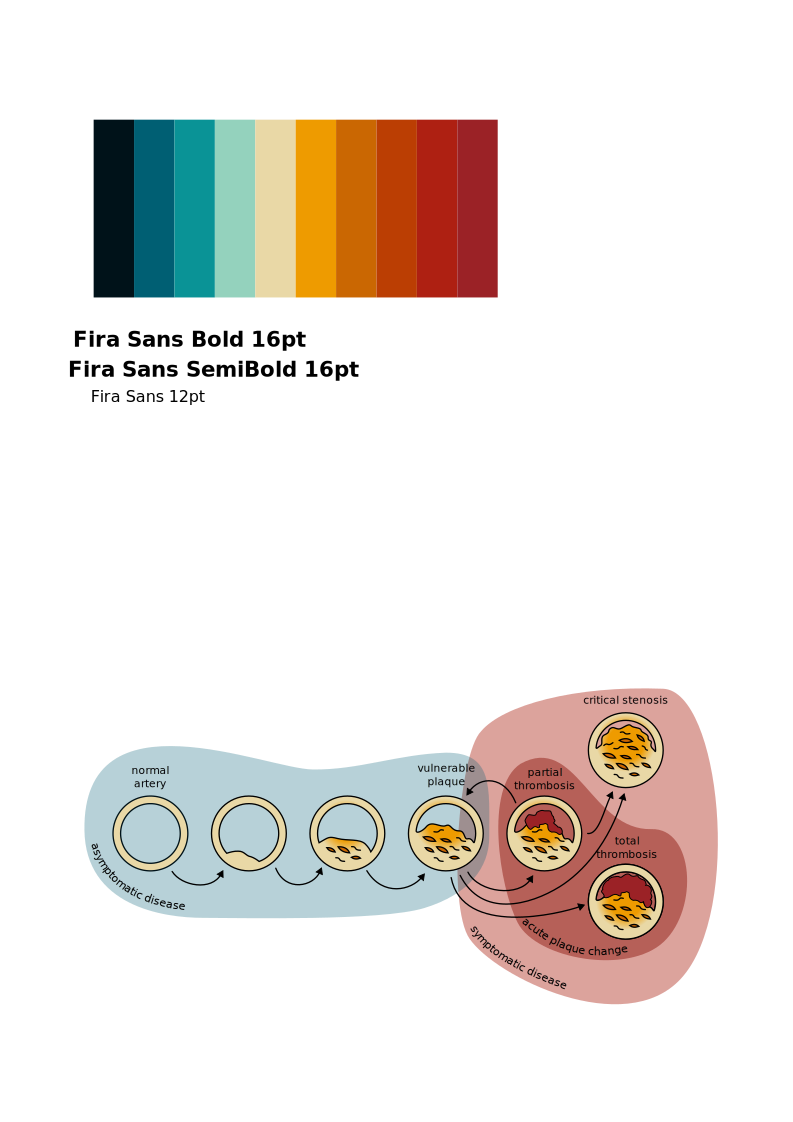
\includegraphics[width=\linewidth]{graphics/atherosclerosis}
    \caption[The process of atherosclerosis]{%
        The atherosclerotic process. 
        From a otherwise normal artery, 
        disruption of endothelial integrity and function, 
        through a combination of genetics and risk factors,
        leads to endothelial injury and low-grade inflammation. 
        Over time, this results in plaque formation through 
        accumulation of lipids, lipoproteins, calcium, and connective tissue.
        Eventually, the plaque may become \enquote{vulnerable}, 
        making it susceptible to sudden rupture or erosion. 
        Such an event can trigger thrombosis and acute changes in the plaque, 
        which, depending on their severity, may either immediately obstruct 
        the arterial lumen%
        ---leading to myocardial infarction or sudden cardiac death---%
        or contribute to further calcification through remodeling. 
        When the progressive narrowing of the arteries reaches a point where 
        it causes symptoms, the stenosis is considered critical, and the 
        myocardium experiences inadequate perfusion, manifesting as 
        ischemic heart disease.
    }
    \vspace{-5.1em}
    \label{fig:atherosclerosis}
\end{figurefw}
\vspace{9em}
% }}}

\section{Disease Manifestation}

The pathological process underlying ischemic heart disease 
is inherently chronic with atherosclerotic lesions 
gradually developing over time, 
but in the event of plaque rupture it can abruptly transition
and manifest as an acute condition.
The clinical presentation of ischemic heart disease  
is consequentially diverse and includes both acute 
~\autocite{byrne20232023}
and chronic coronary syndromes.
~\autocite{knuuti20192020}

Acute coronary syndromes includes 
\ac{UA}, \ac{STEMI}, and \ac{NSTEMI},
that collectively represents a spectrum of acute onset or progression of 
myocardial ischemia.
If the ischemia is sufficient to cause myocardial necrosis, 
it is per definition called \ac{MI}~\autocite{thygesenFourth2019}.
\ac{STEMI} and \ac{NSTEMI} are both forms of \ac{MI} that are distinguised
by a characteristic presence or absence of ST-segment elevation on a \ac{ECG}.
All of the acute coronary syndromes are typically associated 
with acute plaque change and atherothrombosis, 
and are medical emergencies that require immediate 
intervention to limit or prevent myocardial damage.
~\autocite{kumarRobbins2014}

% figure: ecg{{{
\begin{marginfigure}%
    \vspace{1em}
    
\includegraphics{graphics/electrocardiogram}
    \caption[Normal QRS complex]}}

Chronic coronary syndromes are more stable manifestations of the disease,
and include stable angina and chronic ischemic heart disease.
Stable angina, or \textit{angina pectoris}, is characterised by episodes of
crushing chest pain caused by myocardial ischemia, initially typically during
exercise.
By definition, the level of ischemia is not severe enough to lead to
tissue necrosis. 
~\autocite{knuuti20192020}
Unlike \ac{UA}, the symptoms of stable angina are often more predictable,
reliably triggered by a specific level of physical exertion, 
and typically absent when the individual is at rest. 
Chronic ischemic heart disease can either be a long-term progression of stable
ischemic heart disease or a late-stage stabilization following a \ac{MI} that
has undergone revascularization. 
~\autocite{knuuti20192020}
This condition represents the cumulative
effects of prolonged myocardial ischemia and accrued myocardial damage,
ultimately leading to progressive congestive heart failure.
~\autocite{kumarRobbins2014}

\section{Diagnosis and Treatment}

Since the 1950s, a series of groundbreaking scientific advances have improved 
our understanding and management of cardiovascular disease, leading to a 
drastic decline of mortality in ischemic heart disease.
~\autocite{nabelTale2012}
These advances span from from diagnostic imaging techniques to pharmacological
therapies and surgical interventions, each contributing to a more nuanced
understanding of the disease and more effective treatment options.
~\autocite{nabelTale2012}
To translate this constantly evolving body of knowledge into actionable medical
practice, the European Society of Cardiology (ESC) annually releases
comprehensive clinical practice guidelines that cover a wide array of
cardiovascular conditions.

In line with ESC guidelines, 
invasive management is the recommended approach
for immediate treatment of acute coronary syndromes.
This includes primary \ac{PCI}%
% sidenote: pci{{{
\sidenote[][-3em]{%
    \ac{PCI} is a minimally invasive procedure used for treatment of
    atherosclerosis. It involves the use of a small balloon catheter 
    to widen flow-limiting stenoses and restore cardiac perfusion.
} % }}}
for \ac{STEMI} and emergency angiography, 
potentially with concurrent \ac{PCI},
for patients with very high-risk \ac{NSTEMI} and \ac{UA}.
For those with a more stable presentation, but still at high-risk, 
angiography within the first 24 hours is indicated to
assess the need for revascularization. 
~\autocite{byrne20232023}
Based on factors such as the coronary anatomy, 
number and grade of stenotic vessels, 
and the estimated risk of surgical complications
\ac{CABG} is sometimes preferred over \ac{PCI}.
~\autocite{neumann20182019}
The primary objective of these interventions 
is providing timely revascularization where needed,
to restore coronary perfusion and limit myocardial damage.

Contrastingly, for chronic coronary syndromes,
invasive coronary angiography is typically not 
the first-line diagnostic test.
~\autocite{knuuti20192020}
However, for patients with a high clinical likelihood of ischemic heart
disease, who present with easily induceable or refractory angina pectoris 
and a high event risk, coronary angiography is recommended for assessment of
revascularization options.  
~\autocite{knuuti20192020}

Concurrent with invasive treatment, 
the guideline gives a class I recommendation for initiation 
of antithrombotic therapy in patients with \ac{IHD}. 
~\autocite{byrne20232023}
While the specifics of this therapy is beyond the scope of this thesis,
it generally involves a combination of antiplatelet medications, 
aimed at preventing further thrombotic events.
~\autocite{nabelTale2012}

\section{Secondary Prevention}

%% marginnote {{{
\marginnote[-2.5em]}}

Once the acute phase of the disease has been stabilized 
through revascularization or other treatments,
the clinical focus shifts to long-term management and secondary prevention.
Patients with established ischemic heart disease are generally of 
high risk of subsequent events, 
particularly if risk factors are not adequately managed.
~\autocite{clarkMetaAnalysis2005}
Guidelines advocate for a multifaceted approach to secondary prevention, 
incorporating lifestyle changes like quitting smoking and starting exercise, 
as well as pharmacological interventions such as lipid-lowering therapies. 
~\autocite{visseren20212021}

The goal of long-term treatment is essentially twofold:
to limit the progression of existing atherosclerotic plaque and 
to prevent and limit thrombus formation if plaques should rupture or erode.
~\autocite{foxMyth2020}
The clinical trajectories of patients with chronic manifestations of 
ischemic heart disease can remain stable for several years,
before unexpectedly deteriorating to 
major adverse cardiovascular events.
~\autocite{foxMyth2020}
Consequently, continuous monitoring and risk factor control 
are recommended to guide secondary prevention therapy.

In this setting,
risk stratification models that combine the clinical characteristics 
and risk factor profiles of the individual patient can be useful.
~\autocite{visseren20212021}
These models could help identify at-risk patients most likely to benefit from 
aggressive therapy. 
However, the real-world application of such models is not without challenges.
There is a need for rigorous validation studies to establish their 
clinical utility, as well as the development of 
protocols for their integration into routine clinical practice.

Additionally, there is a gap in understanding how comorbidities---%
whether cardiovascular or non-cardiovascular---%
affect outcomes and should be factored into treatment planning and prognosis.%
\sidenote[][13em]{\cite{visseren20212021}}
This is where the role of precision medicine becomes particularly salient. 
By leveraging advanced computational techniques and large-scale clinical data,
precision medicine has the potential to fill these gaps.

\section{Perspectives of Precision Medicine}

A 2013 Cochrane review on \citetitle{taylorStatins2013} concluded 
that statins effectively lower all-cause mortality and reduce the incidence
of both fatal and non-fatal cardiovascular events without any serious
adverse effects~\autocite{taylorStatins2013}.
For instance, the relative risk of fatal cardiovascular events 
when using statins as opposed to placebo
was estimated to \num{0.82} with a 
\si{95}{\%} \ac{CI} of \num{0.70} to \num{0.96}.
~\autocite{taylorStatins2013}
This suggests those treated with statins, on average,
are \si{18}{\%} less likely to die from cardiovascular causes. 
However, it is important to emphasize that this \si{18}{\%} 
reduction is an average effect for the \enquote{average individual}.
There might be groups of people for whom the reduction could be 
even higher, while others may see little to no benefit. 
Understanding and making use of such individual variability 
is the central objective of \enquote{precision medicine}.

Precision medicine is broadly speaking an approach to healthcare 
that aims to tailor medical treatment and management to the individual patient.
Instead of employing a \enquote{one-size-fits-all} methodology, 
where treatment and preventive care is being developed to the average patient,
precision medicine uses data-driven approaches to also account for 
the specific factors of the individual.
As such, the underlying idea of precision medicine is not really new;
tissue- and blood typing, for example,  
has been used to guide organ and blood donation for several decades.
However, the prospective of leveraging large clinical databases
and broad array of phenotypic information is adding renewed interest 
in the concept.
~\autocite{collinsNew2015}

% table: pgx-vars {{{
\begin{table*}[t]
\footnotesize
\centering
\tlfstyle
\begin{tabularx}{\linewidth}{r l p{3cm} X p{3.1cm}} 
\toprule
Gene & Variant & Drug & Description & Reference \\ 
\midrule

ABCG2 
& rs2231142
& rosuvastatin 
& Genotypes GT and TT is associated with increased plasma concentrations of 
rosuvastatin compared to genotype GG. 
&  \href{https://www.pharmgkb.org/clinicalAnnotation/1451666660}{1451666660}
\\

CYP2C9 
& *2 + *3 
& fluvastatin 
& Heterozygous or homozygous mutant allele carriers (*2 or *3) 
have an increased plasma concentration of fluvastatin.
& \href{https://www.pharmgkb.org/clinicalAnnotation/1451666740}{1451666740}
\\

CYP2C9 
& *2 + *3 
& fluvastatin 
& Heterozygous or homozygous mutant allele carriers (*2 or *3) 
have an increased likelihood of adverse events
when treated with fluvastatin compared to CYP2C9 *1/*1. 
&  \href{https://www.pharmgkb.org/clinicalAnnotation/1451678600}{1451678600}
\\

SLC01B1 
& rs4149056 
& rosuvastatin, simvastatin, pravastatin, lovastatin, fluvastatin, atorvastatin
& Genotypes CC and CT is associated with an increased risk of myopathy
when treated with either of the listed statins compared to genotype GG.
& \href{https://www.pharmgkb.org/clinicalAnnotation/1451357200}{1451357200},
\href{https://www.pharmgkb.org/clinicalAnnotation/1451244720}{1451244720},
\href{https://www.pharmgkb.org/clinicalAnnotation/1451244740}{1451244740},
\href{https://www.pharmgkb.org/clinicalAnnotation/1043880818}{1043880818},
\href{https://www.pharmgkb.org/clinicalAnnotation/655384011}{655384011},
\href{https://www.pharmgkb.org/clinicalAnnotation/1451465324}{1451465324}
\\

\bottomrule
\end{tabularx}
\caption[Pharmacogenomics of statins]{
	Examples of pharmacogenomics variants related to statin treatment 
	from the PharmGKB database.
	The included variants are all Level 1A clinical annotations, 
	which specify combinations of genetic variants and drugs for which there 
	is targeted prescribing guidance available either in
	current clinical guidelines or in FDA-approved drug labels. 
	Additionally, the Level 1A annotations are required to have a
	minimum of one supporting published article, in addition to the
	variant-specific recommendations.
 }
\label{tab:pgxvars}
\end{table*}% }}}

In the context of statin treatment,
this class of medication is generally both
highly effective and very well-tolerated, with limited side effects.
~\autocite{taylorStatins2013}
Some individuals may experience mild side effects such as muscle aches, 
while more severe side effects like myopathy or rhabdomyolysis 
are exceedingly rare.
~\autocite{thompsonStatinAssociated2003}
The underlying mechanism of 
statin-induced skeletal muscle side effects
is not well defined, 
but appears to be connected with the drug's serum concentration.
~\autocite{thompsonStatinAssociated2003}
Pharmacogenomics, a critical component of the pharmacological aspects of 
precision medicine, 
adds another layer to this understanding. 
It explores how genetic factors influence drug response, 
allowing for understanding etiology and more nuanced treatment plans. 
Genome-wide analyses have already identified \acp{SNP} 
that are associated with an increased risk 
of statin-induced side effects (Table \ref{tab:pgxvars}).
~\autocite{searchcollaborativegroupSLCO1B12008}
~\autocite{thornPharmGKB2013}
Through targeted screening of such genetic variants, 
and considering concurrent medication 
and experiential variability of the patients, 
it might be possible to refine medication regimens 
to maximize efficacy while minimizing side effects---%
a practical application of precision medicine.

Pharmacogenomics is an important step on the way,
but as such it is only one of the \enquote{building blocks} 
of precision medicine.
To fully realize the promise of precision medicine, 
we need a more holistic approach that consider not
only genetics but the multitude of other factors that 
can and will influence the ideal course of treatment.
Figure \ref{fig:precision-cardiology} shows a schematic of 
how such a precision cardiology workflow could look like.

% figure: precision cardiology {{{
\begin{figure}[bth]
    \vspace{1em}
    \caption[Schematic of Precision Cardiology]{%
    Schematic of a precision cardiology workflow.
    Patient characteristics encompass the full range of available data,
    including the individual's entire health and disease history.
    This information resides in an \ac{EHR} database, 
    which also holds data from other patients. 
    The \ac{EHR} database is a valuable research resource, 
    that can contribute to a curated clinical knowledge base. 
    Patient data, the \ac{EHR} database, 
    and the knowledge base is used as input 
    by computational algorithms and tools. 
    These tools act as clinical decision support systems, 
    providing prognostic and diagnostic models. 
    The outputs of these models 
    are shared with both the patient and the physician, 
    facilitating personalized treatment 
    through shared decision-making.%
    }
	\includegraphics{graphics/precision-cardiology}
    \label{fig:precision-cardiology}
    \setfloatalignment{t}
    \vspace{-3em}
\end{figure}
% }}}

The central elements of this precision cardiology workflow is:
\begin{enumerate*}
    \item big data collection and organization
    \item computer-based clinical tools and algorithms
    \item implementation of these tools in clinical decision making
\end{enumerate*}.
In the research underlying this thesis, 
the primary emphasis have been on (i) and (ii),
but without (iii) the advances of precision medicine
will remain mostly academic in scope.
The challenges and future perspectives of the clinical implementation
will be discussed later in the thesis.
Focusing on the first two elements, 
how do we derive tools and algorithms from big datasets?

       % [X]
% \chapter{Fundamentals of Machine Learning and Neural Networks}
\label{ml-fundamentals}

In modern medicine, 
ever increasing amounts of data 
is continuously being generated and collected.
Ranging from structured administrative data 
used primarily for billing purposes
to advanced imaging and high-througput \enquote{omics} analyses,
the array of available data is as diverse as it is plentiful.
Making sense and making use of such massive amounts of data 
necessitates automated methods for data analysis.

% figure: hierarchy of artificial intelligence {{{
\begin{marginfigure}[3em]
    \centering
	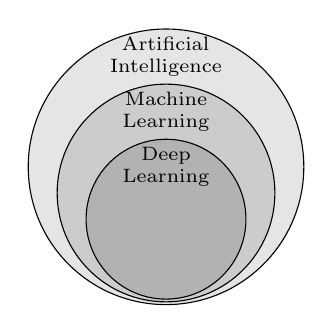
\begin{tikzpicture}[scale=1.75]
        \draw[black, fill=black!10] (0,  0.00) circle (1.00);
        \draw[black, fill=black!20] (0, -0.19) circle (0.79);
        \draw[black, fill=black!30] (0, -0.38) circle (0.58);
        \node[font=\scriptsize, text width=1.8cm, align=center] 
            at (0, 0.8) {Artificial Intelligence};
        \node[font=\scriptsize, text width=1.8cm, align=center] 
            at (0, 0.4) {Machine Learning};
        \node[font=\scriptsize, text width=1.4cm, align=center] 
            at (0, 0.0) {Deep Learning};
	\end{tikzpicture}
    \caption[The hierarchy of artificial intelligence (AI)]{%
        \Ac*{AI} is an umbrella term for computer software 
        that have some sort of \enquote{intelligence} and
        \ac*{ML} is a collection of methods through which 
        that can be achieved. 
        \Ac*{DL}, a specific method in \acs*{ML}, 
        relies on neural networks with many layers
        to analyse complex data.
    }
    \label{fig:artificial-intelligence}
\end{marginfigure}% }}}

\Ac{AI}, and specificically \ac{ML} (\cref{fig:artificial-intelligence}),
seeks to address this need by development of methods and algorithms
that allows computers to \enquote{learn} from data to solve new problems
instead of them being explicitly programmed.
~\autocite{goodfellow2016deep}
The field of \ac{ML} have progressed exponentially
over the past couple of decades, 
and with the advent of generative \ac{AI} models like 
GPT-4~\autocite{openaiGPT42023} and
DALL-E~\autocite{rameshZeroShot2021}
there is a growing public interest in the use of \ac{AI} and \ac{ML}.
In the context of precision medicine,
the promise of \ac{AI} lies in the ability 
to integrate large amounts of data from huge data sets
and register and highlight patterns with clinical importance.
In his review on artificial intelligence in medicine%
\autocite{topolHighperformance2019}, 
Eric Topol expresses his view, that in the not so distant future
\blockquote{%
almost every type of clinician, ranging from specialty doctor to paramedic,
will be using AI technology, and in particular deep learning}.

The underlying principle of \ac{ML} is to formulate a learning problem with a
well-defined objective and a quantifiable measure of performance.
~\autocite{murphyMachine2012}
Subsequently,
a loosely defined computer program is established and fed with data
representing said objective.
Guided by the performance metric, \ac{ML}
algorithms iteratively refine the underlying computer program until the
objective is optimally addressed. 
In his 1997 book \citetitle{mitchellMachine1997},
\citeauthor*{mitchellMachine1997} defines this formally as:
\begin{displayquote}[mitchellMachine1997]
   A computer program is said to learn from experience \(E\)
   with respect to some class of tasks \(T\) and performance measure \(P\),
   if its performance at tasks in \(T\), as measured by \(P\), 
   improves with experience \(E\).
\end{displayquote}
Though this conceptual framework is common to all \ac{ML} models, 
the diversity in \ac{ML} arises from not only the specific \ac{ML} algorithm, 
but also choices regarding objectives, performance metrics, and program attributes. 
These selections introduce the myriad variations and nuances within \ac{ML}, 
which can be broadly categorized into two distinct approaches:
supervised learning
and 
unsupervised learning.
~\autocite{murphyMachine2012}

\section{Supervised Learning}

In supervised learning, models are trained on labeled examples---%
a dataset 
\(\mathfrak{D} = \{(\vec{x}_i, y_i) \mid i \in \{1, \ldots, N\}\} \) 
of size \(N\) that contains both input features \(\vec{x}\)
and corresponding correct output values \(y\)
for all the examples in the dataset. 
Here \( \mathfrak{D} \) is typically refered to as the training set.
~\autocite{murphyMachine2012}
The primary aim in supervised learning 
is to learn a function \(f\) that correctly 
maps input data \(\vec{x}\) to output data \(y\), 
i.e. correctly assigns output labels or values
based on the features present in the input data.
When the output is discrete labels or classes, 
the task is called a classification problem.
Conversely, 
if the output is continuous values,
it is called a regression problem.

Illustrating with a supervised learning task in the domain of classification, 
we can consider a database of coronary angiography images that have been 
manually annotated to indicate the presence or absence of critical stenosis 
in any of the coronary arteries. 
In this scenario, 
the output classes are denoted as 
\(y \in \{\textsf{stenosis}, \textsf{no stenosis}\}\), 
and the objective is to classify the images 
into either of these categories based on their pixel values.
The labeled data is being used to guide and \enquote{supervise}
the model in order for it accurately accomplish this categorisation.

Two other examples of supervised learning tasks is presented in 
\nameref{chap:paper-2} and 
\nameref{chap:paper-3}
within this thesis.
However, these tasks differ from classical supervised learning
in that they involve time-to-event predictions and censored labels.
This subject matter will be elaborated upon in the next chapter:
\nameref{survival-analysis}.

\section{Unsupervised Learning}

In contrast to supervised learning,
unsupervised learning is concerned with finding 
underlying patterns or structures within unlabeled datasets. 
In this paradigm, the algorithm operates without the aid of 
predetermined labels or categories, instead learning from the data itself. 
The aim is to discover intrinsic structure in the dataset, 
which can then be used for tasks such as 
dimensionality reduction, clustering, or anomaly detection.
\sidecite[-8em]{murphyMachine2012}

A canonical example of unsupervised learning is the problem of clustering,
where the objective is to partition a set of objects into subgroups based
on similarity.
\sidecite[-11em]{murphyMachine2012}
Things that are similar should be grouped together and
should be relatively dissimilar to things in other groups.
Defining what constitutes \enquote{similar} 
is therefore a central challenge in clustering;
different measures of similarity often result
in fundamentally different clusterings.%
% card clustering analogy{{{
\sidenote[][-15em]{%
    To illustrate, we can consider a set of playing cards,
    that for convenience is limited to aces, court cards, and tens. 
    One possible clustering groups the cards by suit:
\begin{equation*}
    \begin{array}{@{}c@{}ccccc}
    \{
    &\{ 10\twemoji{heart suit}, 
    &    J\twemoji{heart suit}, 
    &    Q\twemoji{heart suit}, 
    &    K\twemoji{heart suit}, 
    &    A\twemoji{heart suit}
    \}, \\
    &\{ 10\twemoji{spade suit}, 
    &    J\twemoji{spade suit}, 
    &    Q\twemoji{spade suit}, 
    &    K\twemoji{spade suit}, 
    &    A\twemoji{spade suit}
    \}, \\
    &\{ 10\twemoji{diamond suit}, 
    &    J\twemoji{diamond suit}, 
    &    Q\twemoji{diamond suit}, 
    &    K\twemoji{diamond suit}, 
    &    A\twemoji{diamond suit}
    \}, \\
    &\{ 10\twemoji{club suit}, 
    &    J\twemoji{club suit}, 
    &    Q\twemoji{club suit}, 
    &    K\twemoji{club suit}, 
    &    A\twemoji{club suit}
    \}\}
\end{array}
\end{equation*}
Another equally valid clustering groups them by rank:
\begin{equation*}
    \begin{array}{@{}c@{}cccc}
\{ 
   &\{10\twemoji{heart suit},
   & 10\twemoji{spade suit}, 
   & 10\twemoji{diamond suit}, 
   & 10\twemoji{club suit}
\}, \\
   &\{J\twemoji{heart suit}, 
   &  J\twemoji{spade suit}, 
   &  J\twemoji{diamond suit}, 
   &  J\twemoji{club suit}
\}, \\
   &\{Q\twemoji{heart suit}, 
   &  Q\twemoji{spade suit}, 
   &  Q\twemoji{diamond suit}, 
   &  Q\twemoji{club suit}
\}, \\
   &\{K\twemoji{heart suit},
   &  K\twemoji{spade suit},
   &  K\twemoji{diamond suit},
   &  K\twemoji{club suit}
\}, \\
   &\{A\twemoji{heart suit},
   &  A\twemoji{spade suit}, 
   &  A\twemoji{diamond suit}, 
   &  A\twemoji{club suit}
\}\}
\end{array}
\end{equation*}
The choice between these clusterings depends on whether
suits or ranks are considered more important,
which probably depends on the specific card game in question.
This challenge applies to most clustering problems---%
the ideal clustering is usually highly context dependent.
}
% }}}
Clustering lies at the heart of precision medicine:
By identifying distinct subgroups of patients with varying risk profiles, 
clinicians can tailor prevention and treatment strategies more effectively, 
optimizing healthcare outcomes as a result.

In \nameref{chap:paper-1} of this thesis,
we present an example of clustering analysis of patients with 
ischemic heart disease by considering the patterns of comorbidity 
common in subgroups of patients.
The specific methods used in this work is outlined 
in the chapter \nameref{chap:outline-paper-1}.

\section{Generalization and Overfitting}
\label{overfitting}

% figure: generalization error {{{
\begin{marginfigure}[3em]
    \centering
	\includegraphics{graphics/overfitting-2}
    \caption[Overfitting as Function of Number of Epochs]{%
        Training a neural network model for many iterations 
        runs the risk of overfitting the model to the training data.
        Although the training error keeps decreasing, 
        it happens at the expense of increased generalization error.
        Inspired by \cite{goodfellow2016deep}.
    }
    \label{fig:generalization-error}
\end{marginfigure}
% }}}

Returning to supervised learning,
it is important to note that achieving good performance on the 
training set is not the sole objective.
For a \ac{ML} model to be of utility, 
it should maintain its accuracy
when applied to unseen data.
This concept is known as \textit{generalization} and
is a central problem in supervised learning---%
especially when dealing with highly flexible models 
such as neural networks.
~\autocite{goodfellow2016deep}
We can keep track of a model's generalization error 
by introducing an additional dataset, 
that is kept separate from the training set. 
This additional set of labeled examples is refered to as the test set
and is exclusively used for evaluation of model performance.
Assuming that the test set is representative%
\sidenote{%{{{
    An underlying assumption is that the two datasets are 
    independent and identically distributed 
    (typically abbreviated as i.i.d.),
    and thus share the same underlying \textit{data-generating process}.
    [\cite{goodfellow2016deep}]
},
% }}}
the performance on the test set can be used as an estimate of 
the generalization error since it represents unseen data.


\Cref{fig:generalization-error} shows a theoretical training history 
of a neural network model where the performance is calculated 
on both a training and a test set after each iteration of the training.
Here it is illustrated that 
the training loss is monotonically decreasing 
with increasing number of iterations.
The validation loss is at first also decreasing,
but if training continues for long enough,
at some point it will start to increase instead.
The divergence between training and test set performance 
indicates overfitting:
instead of learning generalizable patterns representative of the underlying 
data-generating process,
the model starts to learn or even memorise
the noise and idiosyncracies of the data that,
although characteristic in the narrow scope of the training set,
would not be representative of neither biology nor disease etiology.
~\autocite{murphyMachine2012}
As a consequence, the test set performance is considerably worse 
than the training set performance.

% figure: overfitting {{{
\begin{figure}[htb]
	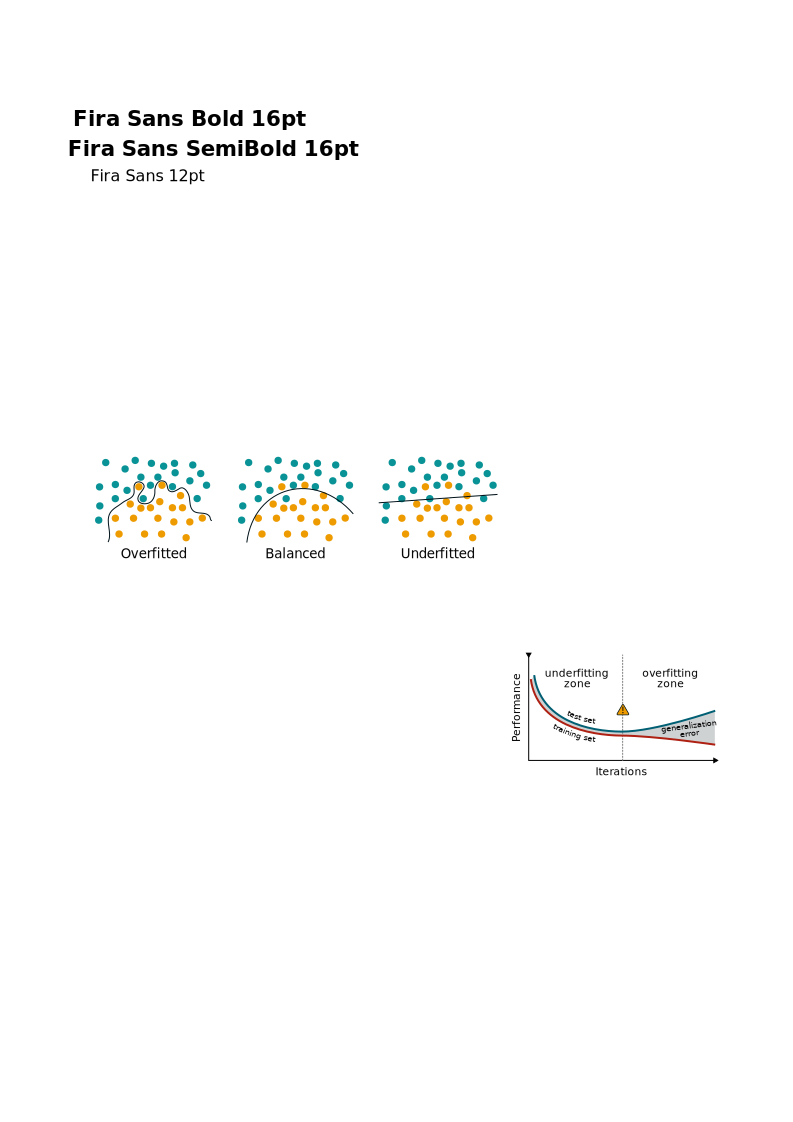
\includegraphics{graphics/overfitting}
    \setfloatalignment{t}
    \caption[What is Overfitting?][-1em]{%
        Illustration of overfitting and underfitting 
        in a simple classification task.
        An overfitted model learns the training data too well,
        and may even remember noise and outliers,
        which makes it perform poorly on unseen data.
        Underfitted models, on the other hand,
        are to simple to capture meaningful patterns in the data.
    }
    \label{fig:overfitting}
    \vspace{-2em}
\end{figure}
% }}}

Overfitting, and its counterpart, underfitting,
are key considerations in training of \ac{ML} models (\cref{fig:overfitting}).
Overfitting happens 
when a model learns the details of the training data too well, 
including the noise, 
which makes it perform poorly on unseen data.
In constrast,
underfitting occurs when the model is too simplistic 
to capture meaningful patterns in the data, 
resulting in poor performance on both the training and test sets.
Both issues highlight the need for balancing the complexity of models,
to ensure that they can effectively generalize to unobserved data.
In the section \nameref{sec:regularization},
I will outline some of the specific methods 
used to balance the complexity 
of neural network models.

\clearpage
\section{Neural Networks}

% figure: neuron{{{
\begin{marginfigure}[3em]
	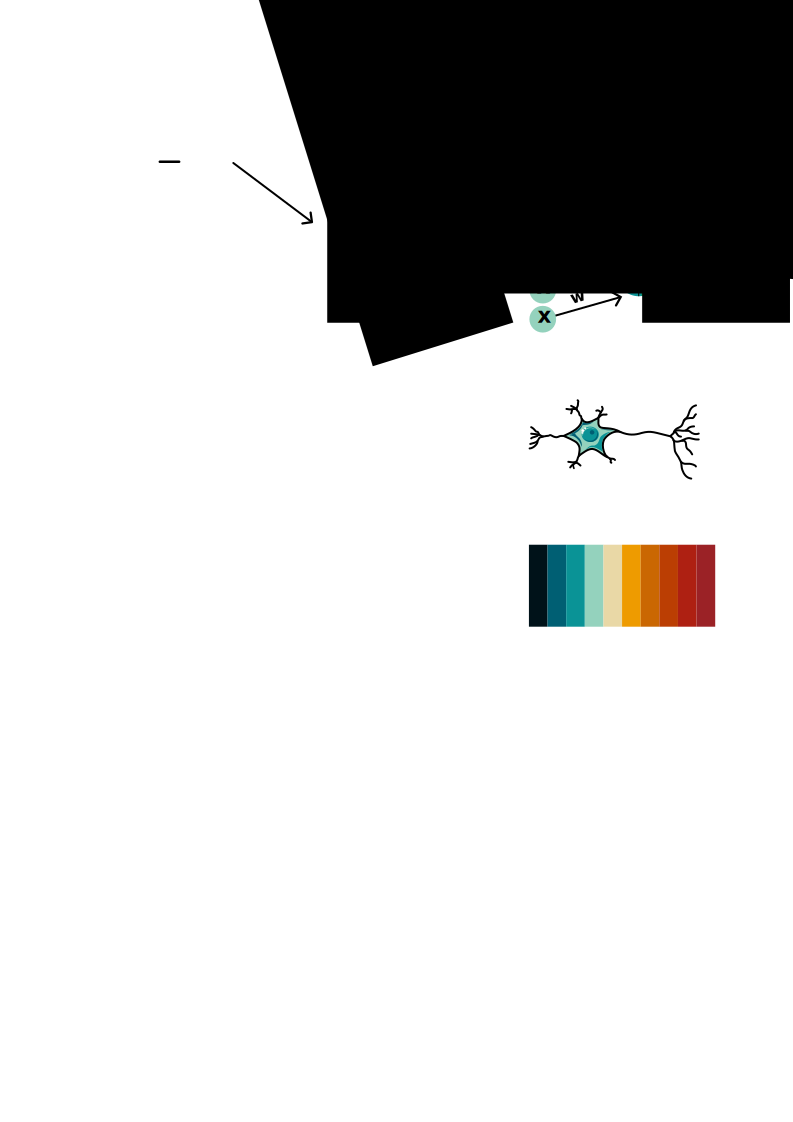
\includegraphics[width=\linewidth]{graphics/neuron}
    \caption[Schematic diagram of a neuron]{%
        Schematic diagram of a neuron.
        A typical neuron has a dendrites, a cell body, and a single axon; 
        the dendrites receive input signals from other neurons,
        and propagates output signals along the axon.
    }
    \label{fig:neuron}
\end{marginfigure}% }}}

In \nameref{chap:paper-2} and \nameref{chap:paper-3}, 
neural network models are utilized to 
develop risk prediction models for ischemic heart disease.
Neural networks is a versatile class of machine learning models
well-suited for handling large and heterogeneous datasets, 
and they currently represent the state-of-the-art in \ac{ML}.
The rest of this chapter will concentrate mainly on neural networks, 
outlining the methodological details and highlight 
relevant practical challenges and considerations 
in their implementation.

Historically, neural networks were designed
using the archicteture of neurons in a human brain as inspiration.
~\autocite{goodfellow2016deep}
The simplest model is that of a perceptron, 
which can be seen as a computational approximation
of a real neuron or nerve cell.
~\autocite{charniakIntroduction2019}
A typical neuron has many dendrites, a cell body, and a single axon 
(\cref{fig:neuron}).
The dendrites carries the input signal to a neuron,
and if the cumulative signal is great enough%
\sidenote[][]{
    This threshold is known as 
    the \textit{threshold potential},
    and is typically between -50 and -55 mV.
}, 
then the neuron will propagate an action potential down the axon%
\autocite{seifterConcepts2005}.
In similar fashion, a perceptron receives may receive many different inputs
and produces a single output (\cref{fig:perceptron}).
In the case of a neuron, the \enquote{all-or-none} principle means
that nerve cells either signals at full strength or not all.
For a perceptron, this principle can be emulated
with the followingly Heaviside step function:
~\autocite{charniakIntroduction2019}

\begin{equation}
    \label{eq:step-function}
    g_{\phi}(\vec{x})  = 
        \begin{cases}
            1 & \text{if } b + \vec{w} \cdot \vec{x} > 0\\
            0 & \text{otherwise}
        \end{cases}
\end{equation}

% figure: perceptron{{{
\begin{marginfigure}%
	\includegraphics[width=\linewidth]{graphics/perceptron}
	\caption{Schematic diagram of a perceptron}
    \label{fig:perceptron}
\end{marginfigure}% }}}

By combing several of such artificial neurons,
in a multilayer-perceptron or feedforward neural network,
we can create a model that, in theory,
can learn even the most complex of patterns.
~\autocite{bishopNeural1995}
In this design (\cref{fig:nn-structure}),
information travels in one direction, from the input layer
through the hidden layers, and finally to the output layer. 
Each layer in a feedforward neural network is
fully connected to the subsequent layer---%
every neuron in one layer is connected to every neuron in the next.

% figure: neural-network {{{
\begin{figure}[tb]
\tikzstyle{node}        =[thick, circle, draw=color0, minimum size=23, 
                          inner sep=0.5, outer sep=0.6]
\tikzstyle{node in}     =[node, fill=color2]
\tikzstyle{node hidden} =[node, fill=color3]
\tikzstyle{node out}    =[node, fill=color4]
\tikzstyle{connect}     =[thick, color0]
\tikzstyle{label}       =[above=0, align=center, font=\sffamily]
\tikzset{ % node styles,
  node 1/.style={node in},
  node 2/.style={node hidden},
  node 3/.style={node out},
}
\def\nstyle{int(\lay<\Nnodlen?min(2,\lay):3)} % map layer number onto 1, 2, or 3
\centering
\begin{tikzpicture}[x=2.0cm, y=1.0cm]
  \readlist\Nnod{6,4,4,4,5}
  \foreachitem \N \in \Nnod{ % loop over layers
    \def\lay{\Ncnt}  % alias of index of current layer
    \pgfmathsetmacro\prev{int(\Ncnt-1)} % number of previous layer
    \foreach \i [evaluate={\y=\N/2-\i; \x=\lay; \n=\nstyle;}] in {1,...,\N}{
      % nodes
      \node[node \n] (N\lay-\i) at (\x,\y) {};
      % connections
      \ifnum\lay>1
        \foreach \j in {1,...,\Nnod[\prev]}{
          \draw[connect, white, line width=1.2] (N\prev-\j) -- (N\lay-\i);
          \draw[connect] (N\prev-\j) -- (N\lay-\i);
        }
      \fi 
    }
  }
  % labels
  \node[label] at (N1-1.90) { Input };
  \node[label] at (N3-1.90) { Hidden Layers };
  \node[label] at (N5-1.90) { Output };
\end{tikzpicture}
\caption[Schematic of a Feedforward Neural Network]{
    A schematic representation of a feedforward neural network, 
    comprising an input layer, multiple hidden layers, and an output layer. 
    Each circle denotes a neuron, and the connecting lines represent 
    connections between neurons.}
\label{fig:nn-structure}
\end{figure}
% }}}

In the context of modern neural networks, 
the simplistic step function in \cref{eq:step-function} 
has certain limitations.
In particular, it is non-differentiable at \(x = 0\) and
has a zero derivative elsewhere, 
rendering it incompatible with gradient-based optimization algorithms.  
To address these issues, other activation functions
have been introduced,
with the sigmoid, \ac{tanh}, and \ac{ReLU} being popular choices 
(\cref{fig:act-fn}), but many other variations exists.
~\autocite{cholletDeep2021}

% figure: activation functions {{{
\begin{figure}[htb]
\pgfplotsset{%
    every axis/.append style={%
        tick label style={/pgf/number format/fixed},
        font=\footnotesize,
        ylabel near ticks,
        xlabel near ticks,
        grid=major
    }}
\centering
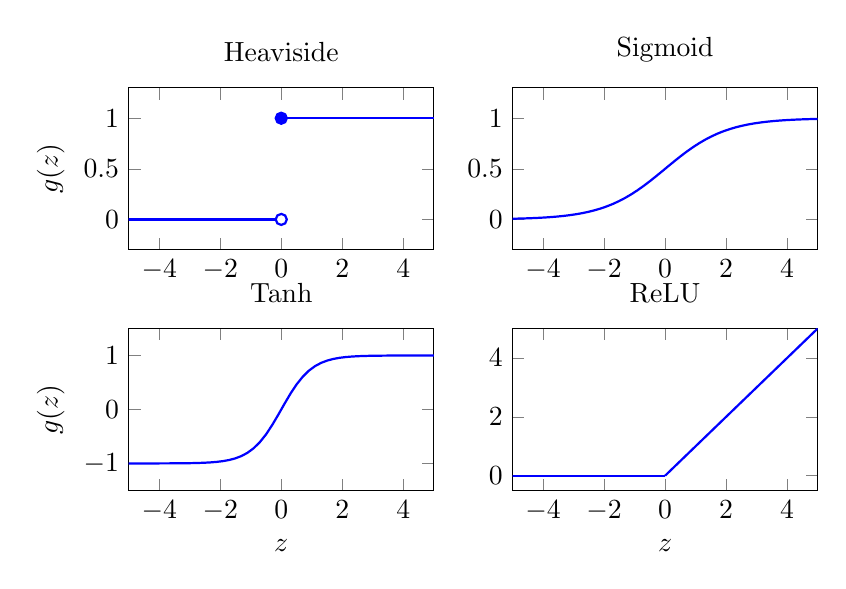
\begin{tikzpicture}% {{{
    \begin{groupplot}[%
        group style={group size= 2 by 2}, 
        width=0.45\linewidth, height=0.30\linewidth
    ]
    \nextgroupplot[
            title=Heaviside, 
            ylabel= \(g(z)\),
            xmin=-5, xmax=5,
            ymin=-0.30, ymax=1.30
        ]
        \addplot[mark=*, blue, thick, samples at={-5.1, 0},
            mark options={fill=white}]  {0};
        \addplot[mark=*, blue, thick, samples at={0, 5.1},
            mark options={}]  {1};
    %% 
    \nextgroupplot[
            title=Sigmoid, 
            xmin=-5, xmax=5,
            ymin=-0.30, ymax=1.30
        ]
        \addplot[domain=-10:10, blue, thick, samples=100] {1/(1+exp(-x))};
    %% 
    \nextgroupplot[
            title=Tanh, 
            ylabel= \(g(z)\),
            xlabel= \(z\),
            xmin=-5, xmax=5,
            ymin=-1.5, ymax=1.5
        ]
        \addplot[domain=-10:10, blue, thick, samples=100] {tanh(x)};
    \nextgroupplot[
            title=ReLU, 
            xlabel= \(z\),
            xmin=-5, xmax=5,
            ymin=-0.5, ymax=5
        ]
        \addplot[domain=-10:0, blue, thick] {0};
        \addplot[domain=0:10,  blue, thick] {x};
        
    \end{groupplot}
\end{tikzpicture}% }}}
\caption[Well-known Activation Functions]{%
    Plots of well-known activation functions used in neural networks. 
    From top left to bottom right: 
    The Heaviside step function, 
    the sigmoid (or logistic) function,
    the \acf{tanh}, and the \acf{ReLU}.
    Each function is plotted against its input value \(z\) 
    to show its respective output \(g(z)\).}
\label{fig:act-fn}
\end{figure}% }}}

In addition to feed forward neural networks, 
ongoing research have developed other neural network architectures 
tailored to particular types of data. 
For example, convolutional neural networks were designed 
for processing image data
~\autocite{lecunHandwritten1989}
and have revolutionized the field of
computer vision.
~\autocite{prince2023understanding}
Similarly, recurrent neural networks,
such as the long short-term memory nework,
can model sequential data
and have had great impact for both time series analysis 
and natural language processing.
~\autocite{hochreiterLong1997}
Another innovation, 
is the introduction of skip or residual connections 
in architectures such as residual networks (ResNet),
which have enabled the training of exceptionally deep networks.
~\autocite{heDeep2015}

\clearpage

\section{Practical Implementation of Neural Networks}

In developing neural network models for \ac{ML} objectives,
several methodological considerations and decisions 
have to be made.
It is not feasible to exhaustively cover
every nuance within the scope of this thesis, 
instead the book \citetitle{goodfellow2016deep} 
serves as a comprehensive reference.%
~\sidecite[-3em]{goodfellow2016deep}
As a guide, 
the following list provides a high-level overview of the typical workflow:%
\sidenote[][-4em]{%{{{
    The list draws inspiration from chapter 19.9 in 
    \cite{russellArtificial2009} and chapter 4 in
    \cite{cholletDeep2021}.
}% }}}

\begin{fullwidth}
%\setcounter{unbalance}{3}
\begin{multicols}{2}
\raggedcolumns
\begin{enumerate}
    \item \label{itm:problem}
        \textit{Problem Definition:} 
        Clearly describe the problem, 
        and in the process identify if the objective belongs to 
        classification, regression, or a third category.
        Attached to the objective should be a measure of performance, 
        which in the neural network literature typically is known as 
        loss function, which is used to direct training.

    \item \textit{Preparing the Data}:

        \begin{enumerate}
        \item \label{itm:data-collection}
            \textit{Data Collection:} 
            Gather and organize data for both training and testing the model.
            Importantly, data should be of reasonable quality,
            pertinent to the problem at hand, and of sufficient quantity.
            If not, it can be a good idea to adjust \cref{itm:problem} 
            to better reflect the available data.

        \item \label{itm:data-preprocessing}
            \textit{Data Preprocessing:} 
            Prepare the data for model training, 
            which may include cleaning, normalization, and transformation tasks.
            The classical saying \enquote{garbage in, garbage out}
            is worth repeating here.
            Any data-informed tasks (e.g. normalization) should exclusively
            be setup using the training set to avoid leakage of data.
            \unskip\footnotemark
        \end{enumerate}

    \item \label{itm:model-specification}
        \textit{Network Structure:} 
        Choose the architecture of the neural network, 
        defining elements such as the number of layers, 
        number of neurons within each layer, 
        and activation functions.
        Certain architectures have shown to be useful for specific 
        types of data, e.g. convolutional neural networks are
        typically the architecture of choice for computer vision tasks.%
        \unskip\footnotemark
        
    \columnbreak
    \item \label{itm:training-specification}
        \textit{Configuring Model Training:}
        \begin{enumerate}%
        \item \label{itm:optimizer}
            \textit{Optimization Algorithm:} 
            Choose and configure an optimization algorithm.
            \Ac{SGD} and variants thereof 
            are the most common algorithms for neural networks,
            \unskip\footnotemark
            and all have different 
            parameters that needs to be defined and possibly tuned 
            (see \cref{itm:hyperparameter}), 
            such as e.g. the learning rate.

        \item \label{itm:regularization}
            \textit{Regularization:} 
            To mitigate overfitting and ensure better generalization,
            consider using regularization techniques such as 
            L1/L2-regularization or Dropout.
            \unskip\footnotemark
        \end{enumerate}

    \item \label{itm:hyperparameter}
        \textit{Hyperparameter Tuning:} 
        Tweak and adjust the relevant hyperparameters specified
        in any of the previous steps,
        including learning rate (from \cref{itm:optimizer})
        and specific details of the neural network architecture 
        (\cref{itm:model-specification})
        to find the best configuration.
        This typically involves training many different intermediate
        versions of the model and evaluating their performance
        using a validation set.

    \item \label{itm:training}
        \textit{Model Training:} 
        Train the final version of the model 
        using the designated training set.

    \item \label{itm:evaluation}
        \textit{Model Evaluation:} 
        Assess the trained model using the test set, 
        calculating metrics like accuracy, precision, and recall 
        to gauge its effectiveness.
        Model explainability techniques can here 
        be helpful in aiding the interpretation of the model.
\end{enumerate}
\end{multicols}
\end{fullwidth}

\footnotetext{\cite{cholletDeep2021}}
\footcitetext{lecunHandwritten1989}
\footcitetext{cholletDeep2021}
\footcitetext{goodfellow2016deep}

While presented as sequential steps, 
the items in the list are almost all interrelated 
and can and should affect one another. 
As an example, 
it especially evident that
\cref{itm:data-collection} 
drastically influences the range of possibilities in 
\cref{itm:problem}.
In the remaining sections of this chapter, 
I will be highlighting select concepts integral to  
building neural network models which have specific
relevance to the papers included in the thesis.

\section{Model Selection}
\label{sec:model-selection}

We can estimate the generalization error of a model
by evaluating it on a test set.
If we are only creating a single model,
then this approach suffices. 
However, we might want to compare many different models,
or slightly tweak an already existing model,
such that we can select the best performing version.
This is particularly relevant in the context of hyperparameter optimization,
a topic that I will return to later in this chapter.
If we select the final model based on the test set alone,
we might inadvertently have biased the process,
and could, in a sense, have overfitted to the test data.
~\autocite{murphyMachine2012}
To avoid this, we need to completely hide away the test data
until we are done with training, experimenting, 
and model selection.
To enable this, a common solution is to introduce a third dataset by splitting 
the training data into two sets of data: a training set and a validation set.
The three sets of data used in the development process is then: 
%
\begin{itemize}
    \item a training set to train or develop candidate models
    \item a validation set to evaluate and select the best model
    \item a test set for the final evaluation of model performance
\end{itemize}

\section{Regularization}
\label{sec:regularization}

Regularization is a collection of strategies used to avoid
overfitting by penalizing the complexity of \ac{ML} models.
Two classical examples are L2 and L1 regularization
that adds an regularization term \(\omega\),
on the model parameters \(\phi\),
to the loss function \(\mathcal{L}\).
~\autocite{goodfellow2016deep}

\vspace{1.5em}
\begin{equation}
    \widetilde{\mathcal{L}} (\vec{\phi} , \mathsf{X}, \vec{y}) =
    \mathcal{L} (\vec{\phi} , \mathsf{X}, \vec{y}) +
    \eqnmarkbox[blue]{node1}{ \omega (\vec{\phi})}
\end{equation}
\annotate[yshift=.5em]{left}{node1}{regularization term}

In the case of L1 regularization, 
the regularization term consists of 
the sum of the absolute values of the model parameters, 
also known as the L1 norm. 
For L2 regularization, 
the term comprises the sum of the squares of the model parameters, 
otherwise known as the squared L2 norm.
~\autocite{murphyMachine2012}
%
\begin{alignat}{3}
    &L1: \quad \omega (\vec{\phi}) 
        &&= \lambda||\vec{\phi}||_1 
        &&= \lambda\sum_{i}|\phi_i|  \\
    &L2: \quad \omega (\vec{\phi}) 
        &&= \lambda||\vec{\phi}||_2^2 
        &&= \lambda\sum_{i} \phi_i^2
\end{alignat}

The regularization strength is controlled by a hyperparameter, \(\lambda\);
a value close to zero imposes minimal regularization, 
while larger values increases the amount.
In the context of neural networks, 
another commonly used regularization method is \textit{dropout}.
~\autocite{srivastava2014dropout}
This method simply involves randomly dropping some of the output features
of the hidden layers during each iteration of the training.
This process in a sense creates a different architecture at every step, discouraging the model from becoming overly dependent on any single feature 
and thereby enhances generalization. 
~\autocite{charniakIntroduction2019}
Empirically, dropout have been found to give significant improvements across
many different architectures 
~\autocite{srivastava2014dropout}
and is a consequence broadly utilized.
~\autocite{charniakIntroduction2019}
The droput rate, which controls the probability \(p\) of dropping out each
individual unit, is a hyperparameter that needs to be specified.

\section{Hyperparameter Optimization}

Neural networks, as well as most other \ac{ML} models,
have parameters and settings that are not adjusted 
during training and therefore needs to pre-specified.
~\autocite{goodfellow2016deep}
These parameters are known as hyperparameters, 
and common examples include aspects such as 
learning rate,
number of layers in the neural network,
number of nodes in each layer,
Other specific examples have also been described previously in this chapter.

Although it is possible to assign default values to hyperparameters 
based on prior experience and personal preference, 
it is imperative to acknowledge their possible impact on model performance.
Consequently, it is common to explore different setting and combinations
of hyperparameters in the model building process.
~\autocite{goodfellow2016deep}
In the field of machine learning, this process is known as \ac{HPO}.

If the number of hyperparameters are sufficiently small,
a commonly employed strategy for \ac{HPO} 
is creating a range of possible candidate values 
for each hyperparameter and 
simply testing the entire space of 
possible combinations in what is known as a \emph{grid search}.
The disadvantage is, however, that the search space quickly 
explodes in size and this strategy may therefore not be feasible.
An alternative strategy, 
which have been emprirically and theoretically shown to outperform
grid search, and therefore typically should be prefered,  
is \emph{random search}.
~\autocite{bergstraRandom2012}
In random search, the hyperparameters values are neither binned nor
discretized and are instead sampled from a uniform distribution.
~\autocite{bergstraRandom2012}
State-of-the-art \ac{HPO} approaches includes Bayesian optimization 
models, multi-fidelity optimization, and metaheuristics algorithms.
~\autocite{yangHyperparameter2020}
Many of these algorithms are implemented in the 
open-source Python package \textit{Optuna},
a very popular software framework for \ac{HPO} in Python.
~\autocite{akibaOptuna2019}

\section{Model Explainability}

As described above, the overall goal of \ac{ML} 
is to make accurate predictions on unseen data,
and the \enquote{how} and \enquote{why} of such predictions is,
in the general \ac{ML} paradigm, 
explicitly of little concern.
Consequently, it is accepted that complex neural networks
with deep architectures and many thousands of parameters 
are \enquote{black box} models that can not 
be easily described nor understood.
~\autocite{russellArtificial2009}
For many applications, 
this lack of transparency can be accepted,
but for other applications where trust is paramount, 
including precision medicine,
ongoing efforts seeks to adress this inherent limitation.
~\autocite{vanderveldenExplainable2022}

In the discussion of \Ac{XAI}, there is 
a meaningful distinction to be made between 
interpretability and explainability:
A model is said to be interpretable if we can 
relatively easily understand the model through inspection
of the model itself.
~\autocite{russellArtificial2009}
An explainable model, on the other hand, is a simplified 
external process that provides an interpretable approximation
of the complex non-interpretable model.
~\autocite{lundbergUnified2017}
For neural networks,
model explainability techniques are generally 
the only available option.

\subsection{What is SHAP Analysis?} 

A popular method for explainability analysis of neural network models
is \ac{SHAP}, first published by
\citeauthor{lundbergUnified2017} in \citeyear{lundbergUnified2017}
~\autocite{lundbergUnified2017}.

The \ac{SHAP} method is based on Shapley values,
a well-known concept from cooperative game theory.
Shapley values is a method for quantifying individual contribution
in cooperative games.
In the context of \ac{ML}, the \enquote{game} is the prediction task
and the \enquote{players} are the model features.



The goal of \ac{SHAP} is to introduce a simple explanation model \(g\),
that approximates the original complex model \(f\) in a manner
such that the model prediction can be represented as a simple sum
of the individual feature contributions.




The Shapley Value is defined as the \(j\)th feature's 
impact on the model output

\begin{equation}
    S_j = \sum_{M} \gamma_n (M) \left[
        \nu (M \cup {j} - \nu (M))
    \right]
\end{equation}








Formally, we let \(f\) refer to the complex model to be explained, 
and introduce an explanation model \(g\) that approximates \(f\).



\begin{equation}
    f(\vec{x}) \approx g(\vec{x})
\end{equation}

\begin{equation}
    g(\vec{x}) 
    = w_{0} + \sum_{j=1}^{m} w_j x_{j}
\end{equation}

These models attribute an effect \(w_j\) to each feature \(x_i\),
and the sum of all feature effects (plus some offset), 
approximates the complex model \(f\).




\ac{SHAP} is an additive feature attribution method, 
which means that 
~\autocite{lundbergUnified2017}.


The \ac{SHAP} method is based on Shapley values,
a well-known concept from cooperative game theory.
Shapley values is a method for quantifying individual contribution
in cooperative games.
In the context of \ac{ML}, the \enquote{game} is the prediction task
and the \enquote{players} are the model features.

One limitation of XAI models is the accuracy and relevance of explanations.
Explainability algorithms such as SHAP are only approximations
of the complete model.
In other words, the fidelity is not perfect and therefore neither
is the explanation.
However, for black-box models such as neural networks,
it is the next best thing.

\subsection{Scope of Explanations}

The scope of an explanation is the difference between
explanations for a complete model and
explanations for a single output.
Global explanation covers feature importance estimates 
for the entire dataset.
Local explanations, on the other hand, seeks to explain
the impact of the specific example under scrutiny.

A SHAP-waterfall plot is an example of a local explanation.
A saliency map of a chest radiograph that shows
which pixels contributed to the label \enquote{liver cancer}
is another example.

Shapley values measures the marginal contribution
of each individual feature.


   % [X]
% \chapter{Time-to-Event Prediction with Neural Networks}
\label{chap:survival-analysis}

\marginnote{%→
    \setlength{\parindent}{0pt}
    \vskip 1em
    What is survival analysis?
    \begin{description}[leftmargin=!, labelwidth=3em]
        \item[outcome] time until an event occurs.
            Can be measured in seconds, days, months, etc.
        \item[event] death, relapse, remission, engine failure, etc.
    \end{description}
    
    \begin{center}
    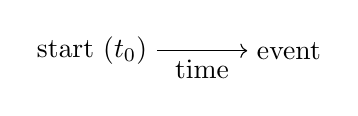
\begin{tikzpicture}
        \noindent
        \node (a) at (2.5, 0) {event};
        \node (b) at (0, 0) {start (\(t_0\))}; 
        \draw[->] (b) -- (a) node[midway, below] {time};
    \end{tikzpicture}
    \end{center}
}% ←

In the prior chapter, 
I provided and  overview of machine learning and neural networks,
highlighting central ideas and concepts releveant to the research presented
in this thesis.
Specifically, neural networks were employed in
were used in \studyii{} and \studyiii{} to develop
prediction models for ischemic heart disease.
These models, however, diverge from classical neural network methods
in that they include adaptions that that render them suitable for
modelling and prediction of time-to-event data.
This chapter delves into the fundamentals of survival analysis,
subsequently detailing the theoretical approaches used for implementing
survival analysis in neural network models.

\section{Introduction to Survival Analysis}

Generally, 
survival analysis is the collection of statistical methods
for the modelling and analysis of time-to-event data,
which is a type of data where the outcome variable of interest 
is the time until \enquote{something} happens.~%
~\autocite{kleinbaumSurvival2011}
This \enquote{something} is a particular event of interest,
which, depending on the type of analytical problem, 
could be cancer relapse, 
diabetes remission,
or death.

In cardiovascular research, 
common examples of time-to-event outcomes include
\begin{enumerate*}
    \item time to death attributed to any cause (all-cause mortality)
    \item time to death due to a specific cause (e.g. sudden cardiac arrest)
    \item time to first occurence of a \ac{MACE}
\end{enumerate*}.

To figure out what processes and characteristics 
that are associated with these events, 
in survival analysis, we try to model the relationship between
explanatory variables and the number of weeks, months, or years 
until that particular event is likely to occur. 

% marginnote→
\marginnote{%
    Survival analysis have applications outside biomedical research.
    In engineering, it is called \textit{reliability analysis} and
    is used to model the time-to-failure of system-critical components 
    such as e.g. bearings or valves.
}% ←

Although this task can be daunting in its own right, 
an additional complication to survival analysis 
is the presence of observations that are subject to 
censoring.
This concept, censoring, refers to cases 
where the event of interest has not been observed 
before the end of follow-up, 
e.g. when a study or experiment has to be stopped.
In such cases, 
we would know that a given subject did not experience a relapse 
in the three months he or she was included in the study, 
but after the study period ends, 
we have no information on the status of the patient. 
Including and utilizing this partial information
is a cornerstone in many survival analysis problems.

There exists different forms of censoring,
such as right censoring, left censoring, and interval censoring.
In the study designs used throughout this thesis 
we have only had to deal with right censoring,
the most common form of censoring,
so the two other types will not be described further.
See instead the text book by \citeauthor{kleinSurvival2003} 
for more details on this.
~\autocite{kleinSurvival2003}

\section{Fundamentals of Survival Analysis}

In survival analysis, 
the central outcome variable is survival time,
a non-negative random variable denoted as \(T\). 
When refering to specific values of \(T\), 
a lower case \(t\) is typically used.  
A survival dataset \(\mathfrak{D}\) of size \(N\) is given by
\begin{equation}
    \mathfrak{D}_N = \{(t_i, \sigma_i, \vec{x}_i) \mid i = 1, \ldots, N\} 
\end{equation}
where \(t_i = \min(T_{i}, C_i) \) is the survival time 
for the \(i\)th subject,
with \(T_i\) denoting the survival time
and \(C_i\) denoting the censoring time. 
Also, \(\vec{x}_i = (x_1, x_2, \dots, x_p)'\) is the covariate vector
and \(\sigma_i\) is the event indicator, which is defined as
\begin{equation}
    \label{eq:sigma-def}
    \sigma_i =
        \begin{cases}
            0 & \text{if subject is censored} \; (T_i >    C_i) \\
            1 & \text{if event is observed} \; (T_i \leq C_i)
        \end{cases}
\end{equation}

In the following, I will initially be assuming that \(T\) is 
continuous and that there is an absence of competing risks, 
however both of these assumptions will later be relaxed in the discussion 
of competing risks and discrete-time survival analysis.

\subsection{Basic Survival Quantities}
\label{sub:survival-quantities}

% figure: theoretical survival function{{{
\begin{marginfigure}%
	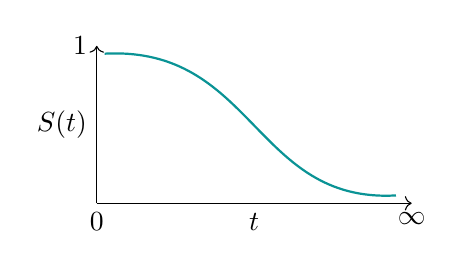
\begin{tikzpicture}[scale=2]
	  \draw[->] (0, 0) --  (2,0) 
		node[pos=0.0, below] {$0$}
		node[pos=0.5, below] {$t$}
		node[pos=1.0, below] {$\infty$};
	  \draw[->] (0, 0) --  (0,1) 
		node[pos=1.0, left] {$1$}
		node[pos=0.5, left] {$S(t)$};
	  \draw[-, color=color2, thick] 
		(0.05, 0.95) .. controls (1, 1) and (1, 0) .. (1.90, 0.05);
	\end{tikzpicture}
    \caption[A theoretical survival function]}}

In survival analysis, 
the central function of interest is 
the survival function \(S(t)\), 
that represents the probability 
of an individual still being alive after 
some specified duration of time, we have that 
%
\begin{equation}
    S(t) = \PR (T > t), \quad 0 < t < \infty.
\end{equation}

The survival function is 
the integral of the probability density function, \(f(t)\),
and is the complement to the cumulative distribution function, \(F(t)\),
which means that
~\autocite{kleinSurvival2003}
%
\begin{equation}
    S(t) = 1 - F(t) 
    \quad \text{and} \quad 
    S(t) = \int_{t}^{\infty} f(u) \, \diff u
\end{equation}

Another fundamental quantity is the hazard function, or hazard rate,
which represents the instantaneous failure rate at a given timepoint,
and is defined as
%
\begin{equation}
    \label{eq:hazard-function}
    \lambda(t) = \lim_{\Delta t \to 0} 
        \frac{\PR (t \leq T < t + \Delta t \mid T \geq t)}{\Delta t}
\end{equation}
% 
from which it can be shown that
~\autocite{kleinSurvival2003}
%
\begin{equation}
    \lambda(t) = \frac{f(t)}{S(t)} = -\frac{\diff}{\diff t} \ln[S(t)].
\end{equation}
%
and thus the hazard function completely describes the distribution of \(T\),
such that all the the other quantities can be obtained from it---%
as well as the other way around.

In terms of its interpretation, 
from \cref{eq:hazard-function} it follows that \(\lambda(t)\Delta t\) 
is a measure of the conditional probability of failure in a small time
window, given that the individual is still alive at time \(t\).
~\autocite{kleinSurvival2003}

Analogous to the relation between \(f(t)\) and \(F(t)\), 
integrating \(\lambda(t)\) with respect to \(t\),
we obtain cumulative hazard function, defined as
%
\begin{equation}
    \Lambda(t) = \int_{0}^{t} \lambda(u) \, \diff u = -\ln[S(t)].
\end{equation}

\subsection{The Kaplan-Meier Estimator}

The survival function of a population
can be estimated using the Kaplan-Meier method,
which is the standard estimator of the survival function.
~\autocite{kaplan1958nonparametric}
~\autocite{kleinSurvival2003}
In order to estimate the survival function, 
in the Kaplan-Meier method we first order
the distinct failure times such that%
\sidenote{%
    Following the example of [\cite{kleinbaumSurvival2011}], 
    the \(t\)'s denoted with subscripts within parentheses \(t_{(j)}\)
    refers to the \(j\)th element of the ordered distinct failure times and
    are thus different from \(t_1, t_2, \ldots, t_i\) that refers to the 
    observed failure time of subject \(1\), \(2\), and \(i\)
}
\begin{equation*}
    t_{(1)} < t_{(2)} < \ldots < t_{(j)},
\end{equation*}
%
and we introduce two quantities to keep track of
the number of failures/events at each timepoint \(\widebar{D}(j)\), 
as well as the number of subjects still at risk at each timepoint \(\widebar{A}(j)\).
They are defined as
\begin{equation}
\begin{aligned}
    \bar{D}(j) &= \card \{i \in \{1, \dots, n\} \mid t_i = t_{(j)}, \sigma_i = 1\} \\
    \bar{A}(j) &= \card \{i \in \{1, \dots, n\} \mid t_i > t_{(j)}\}.
\end{aligned}
\end{equation}

With these two quantities in place, 
the Kaplan-Meier estimator can then be formulated as 
%
\begin{equation}
    \widehat{S}(t)
    =   \prod_{j \mid t_{(j)} \leq t} 
        \frac{
            \bar{A}(j) -
            \bar{D}(j)
        }{
            \bar{A}(j)
        }
    =   \prod_{j \mid t_{(j)} \leq t} 
        1 - \frac{
            \bar{D}(j)
        }{
            \bar{A}(j)
        }.
\end{equation}

While the Kaplan-Meier estimator is very useful 
for estimating the average survival of a population, 
it does not account for the effect of covariates.
Instead, another approach is needed for regression analyses.

\subsection{Cox's Proportional Hazards Model}

To describe and model the relationship between explanatory variables
and time-to-event phenomenons, a widely used statistical model is 
the Cox proportional hazards model. 
~\autocite{coxRegression1972}
This model seeks to model the hazard function over time \(t\),
of an individual with a covariate vector \(\vec{x} = (x_1, x_2, \dots)'\),
and assumes that it takes the form of
%
\begin{equation}
    \label{eq:cox}
    \widehat{\lambda} (t \,|\, \vec{x}) = \hzt \exp [g(\vec{x})],
\end{equation}
%
where \(\hzt\)
is an unspecified baseline hazard function,
and \(g(\vec{x})\) is some parametric function.
For this reason, the Cox model 
is referred to as a semi-parametric model.
In its classical formulation, 
this function is a linear combination of parameters 
\(\vec{\beta}\) and covariates \(\vec{x}\),
as given by

\begin{equation}
    g(\vec{x}) 
    = \vec{\beta}' \vec{x} 
    = \beta_1 x_1 + \beta_2 x_2 + \ldots + \beta_p x_p
\end{equation}

In estimation of the parameters \(\vec{\beta}\),
the baseline hazard \(\hzt\) is treated as a nuisance function
and the coefficients are estimated by
maximising a partial likelihood
in which \(\hzt\) has been abstracted away.
~\autocite{kalbfleischStatistical2002}

A central assumption in the Cox model, 
at least in the standard version with fixed covariates
(\(\vec{\beta}\) instead of \(\vec{\beta}(t)\)),
is that of proportional hazards.
Let \(\vec{x}\) and \(\vec{x}'\) be two different 
covariate vectors, now the ratio between their
respective Cox-estimated hazards is

\begin{equation}
    \label{eq:hazard-ratio}
    \begin{aligned}
    \frac%
        {\widehat{\lambda}(t \,|\, \vec{x} \hfill)}%
        {\widehat{\lambda}(t \,|\, \vec{x'})}
    &=
    \frac%
        {\hzt \exp (\vec{\beta}\cdot\vec{x}\hfill)}%
        {\hzt \exp (\vec{\beta}\cdot\vec{x'})} \\
    &=
    \frac%
        {\exp (\vec{\beta}\cdot\vec{x}\hfill)}%
        {\exp (\vec{\beta}\cdot\vec{x'})} \\
    &= \exp (\vec{\beta} \cdot (\vec{x} - \vec{x'}))
    \end{aligned}
\end{equation}

Since the right-hand side of the equation does not include a term for \(t\),
the hazard ratio between the two samples are constant and 
they are thus proportional to one another.
This shows that by assuming the hazard takes the form of \cref{eq:cox},
then it is also assumed that the hazards between two subjects are proportional.
Although this assumption is a strong one, 
and the validity of the Cox model relies on it, 
the assumption makes interpretation of parameters easier.
~\autocite{tutzModeling2016}
For example, 
in an randomized clinical trial
studying the survival effect of a new type of medication, 
we can let \(x = 1\) represent the experimental treatment  
and \(x' = 0\) represent standard of care, 
then the hazard ratio in \cref{eq:hazard-ratio} takes the form of
%
\begin{equation}
      \exp \left(\beta (x - x')\right)
    = \exp \left(\beta (1 - 0)\right)
    = \exp (\beta ),
\end{equation}
%
which means that if \(\beta < 0\), 
then the hazard of the experimental treatment is 
\(\exp({\beta})\) times lower than standard of care
and should therefore be preferred.%
\sidenote{% 
This example is a slightly modified version of the 
one given in \cite[pp. 50]{tutzModeling2016}}


\section{Time-to-Event Prediction}

Up until now, 
I have outlined various concepts foundational to survival analysis,
focusing primarily on quantities and statistics of time-to-event outcomes
at a population level.
These measures play an important role in understanding 
and interpretation of survival data.

In the context of precision medicine, however,
the emphasis shifts towards making individualized predictions
taking distinct patient-level characteristics into account.
Consequently, as described in \cref{chap:machine-learning}, 
the primary concern lies in 
making accurate predictions on unseen data,
rather than in the exploration of disease etiology and underlying mechanisms.

For prediction of time-to-event outcomes, classical approaches 
include models based on the previously presented semi-parametric Cox model 
as well as various parametric survival models, 
such as those based on exponential, Weibull, or log-normal distributions.
~\autocite{kleinSurvival2003}
This thesis, however, 
explores the use of contemporary machine learning methods 
in time-to-event prediction,
with a particular emphasis on the application of neural networks.

\subsection{Neural Networks and Time-to-Event Outcomes}

The first application of neural networks for time-to-event prediction
was demonstrated by
\citeauthor{faraggiNeural1995} in
\citeyear{faraggiNeural1995},
and involves parameterising the parametric part of the Cox model
with a neural network, 
such that the \(g(\vec{x})\) term in \cref{eq:cox} is a 
flexible neural network model instead of a simple linear function.
\autocite{faraggiNeural1995}

\vspace{.5em}
\begin{equation*}
    \widehat{\lambda} (t \,|\, \vec{x}) = \hzt \exp [
    \eqnmarkbox[color2]{node1}{
        g(\vec{x})
    }]
\end{equation*}
\annotate[yshift=.6em]{left}{node1}{use neural network}

This approach was later further refined
in the \emph{DeepSurv} paper from 
\citeyear{katzmanDeepSurv2018a},
in which modern neural network techniques
were added to Faraggi-Simon framework, 
which markedly improved its usefulness.
~\autocite{katzmanDeepSurv2018a}
\citeauthor{katzmanDeepSurv2018a} showed that the flexibility 
offered by neural networks led to increased performance
in both synthetic and real-life time-to-event prediction applications
compared to a standard Cox model.
However, the \emph{DeepSurv} approach is still limited by the 
assumption of proportional hazards.

\subsection{Overview of Approaches}

Recently, there have been considerable interest in neural network-based
time-to-event prediction models, and as a consequence, many new methods 
have since been developed.
For a thorough overview of the existing approaches, 
\textcite{wiegrebeDeep2023} and 
\textcite{kvammeContinuous2021} provide valuable insights.
Generally, two prevailing types of approaches exists:
continuous-time methods based on the Cox model, 
which includes \emph{DeepSurv},
and discrete-time methods as exemplified by 
\textcite{leeDeepHit2018} and \textcite{gensheimerScalable2019}.

The discrete-time approaches offer several advantages that 
make them particularly relevant for neural network. 
Furthermore, they have been shown to offer better predictive
performance compared to the Cox-based methods.
~\autocite{kvammeContinuous2021, leeDeepHit2018, gensheimerScalable2019}
Notably, \emph{DeepHit}\autocite{leeDeepHit2018}
and \emph{Logistic-Hazard}\autocite{gensheimerScalable2019}
are the two most cited papers in this context as of the time of writing.
Among these and other tested approaches,
\textcite{kvammeContinuous2021} found that 
DeepHit offers excellent discrimination but suffers from poor calibration.
In contrast, the Logistic-Hazard model have nearly as good discrimination
and also significantly better calibration. 
Consequently, the Logistic-Hazard model, and an extension hereof, 
was chosen for application in 
\studyii{} and \studyiii{}.

In the following section, I will be giving a brief description of
this discrete-time formulation of time-to-event analysis and 
elaborate on the Logistic-Hazard model in more detail.

\section{Discrete-Time Survival Analysis}
\label{sec:disctime-survival}

Most textbooks on survival analysis treats survival time as continuous, 
and that is also usually the case across the biomedical litterature.
However, handling time as a something discrete can be advantegous.
In practice, most measurements of time is inherently discrete 
with durations being recorded in, for example, days; months; and weeks.
The continuous time approaches presented earlier in this chapter, 
are also applicable to discrete time data,
however, methods designed specifically for discrete time-to-event 
data have some advantages~\autocite{tutzModeling2016}:

\begin{itemize}
    \item If observed event times are inherently discrete, 
        then modelling them as such is arguably more appropriate. 
    \item In the discrete-time setting, hazards can be formulated as 
        conditional probabilities which are much more intuitive to 
        both interpret and understand.
    \item Discrete time-to-event models are more easily transferred to 
        other more general purpose modelling frameworks 
        such as generalized linear models, random survival forests, 
        neural networks.
\end{itemize}

The latter point is the main motivation behind both 
the \emph{DeepHit} and \emph{Logistic-Hazard} approach.
For a complete overview of the theory enabling these two approaches,
the book by \textcite{tutzModeling2016} is a valuable resource, 
and serves as the main source of reference for the following.

\subsection{Notation and Definitions}

In the discrete-time framework, 
continuous follow-up time \(\Tic\) is divided into \(q\) contiguous intervals,
that is
%
\begin{equation*}
	(0, a_1], (a_1, a_2], \dots, (a_{q-1}, a_q]
\end{equation*}
%
and \(\Tid \in \{1, \dots, q\}\) is a discrete random  variable
such that if \(\Tid = \tid\) is observed, then the event 
falls in the interval \((a_{\tid-1}, a_{\tid}]\).
Similarly, the discretized censoring time is \(\Cid \in \{1, \dots, q\}\).

With this discrete time scale, 
the distribution of \(\Tid\), 
given some vector of covariates \(\vec{x}\),
can be described using discrete equivalents of the previously 
outlined basic quantities of survival analysis, that is
%
\begin{align}
    \text{probability mass function:} \qquad
    f(\tid \giv \vec{x}) 
    &= \PR (\Tid = \tid \mid \vec{x}) \\
    %
    \text{cumulative mass function:} \qquad
    F(\tid \giv \vec{x}) 
    &= \PR (\Tid \leq \tid \mid \vec{x}) \\
    %
    \label{eq:discrete-hazard}
    \text{hazard function:} \qquad
    \lambda(\tid \giv \vec{x}) 
    &= \PR (\Tid = \tid \mid \Tid \geq \tid, \vec{x}) \\
    %
    \text{survival function:} \qquad
    S(\tid \giv \vec{x}) 
    &= \PR (\Tid > \tid \mid \vec{x})
\end{align}

\subsection{The Logistic-Hazard Model}

\Citeauthor{gensheimerScalable2019}'s approach, 
which they refer to as \enquote{Nnet-survival},
~\autocite{gensheimerScalable2019}
is more accurately characterized as the Logistic-Hazard method, 
as described in \textcite{kvammeContinuous2021}.
In the Logistic-Hazard method, 
the time-to-event data is described by 
modelling the effect of covariates on the discrete hazard function 
(\cref{eq:discrete-hazard}) 
using a neural network.
The concept is not novel, 
employing the discrete hazard for statistical modeling is a common method, 
as covered extensively in \textcite{tutzModeling2016}. 
In addition, a neural-network based model with the same general idea 
was presented by \citeauthor{brownUse1997} in 1997.
~\autocite{brownUse1997}
However, 
\citeauthor{gensheimerScalable2019} were the first to adapt the approach
to current neural network methodologies.

\subsection{Log-Likelihood of the Discrete Hazard}

Let \(\mathfrak{D}_{\mathrm{d}}\) 
be a discrete-time survival dataset of size \(N\),
\begin{equation}
    \mathfrak{D}_{\mathrm{d}} = 
    \{(\tid_i, \sigma_i, \vec{x}_i) \mid i = 1, \ldots, N\},
\end{equation}
where \(\tid_i\) is the discretized survival time, 
\(\sigma_i\) is the event indicator as defined in \cref{eq:sigma-def},
and \(\vec{x}_i = (x_1, x_2, \dots, x_p)'\) is the feature vector.
With the assumption of \emph{noninformative censoring},
~\autocite{kalbfleischStatistical2002}
in the Logistic-Hazard model, 
the contribution of the \(i\)th individual to the likelihood function
can be shown to be  
~\autocite{tutzModeling2016}
\begin{equation}
    \Lik_i = %
    \begin{cases}
        \PR (\Tid_i = \tid_i) & \text{if non-censored} \\
        \PR (\Tid_i > \tid_i) & \text{if censored}.
    \end{cases}
\end{equation}

These two probabilities can be expressed using the discrete hazards,
as it can be seen that
\begin{align}
    \begin{split}
    \PR (\Tid = \tid) 
    &= \PR (\Tid = \tid \mid \Tid \geq \tid) \PR (\Tid  \geq \tid) \\
    &= \PR (\Tid = \tid \mid \Tid \geq \tid) \PR (\Tid  > \tid - 1) \\
    &= \lambda (\tid) \, \prod_{s=1}^{\tid - 1} (1 - \lambda(s))
    \end{split} \\
    \intertext{and similarly}
    \begin{split}
    \PR (\Tid > \tid) 
        &= \PR (\Tid > \tid \mid \Tid \geq \tid) \PR (\Tid  \geq \tid) \\
        &= (1 - \PR (\Tid = \tid \mid \Tid \geq \tid)) \PR (\Tid  \geq \tid) \\
        &= (1 - \PR (\Tid = \tid \mid \Tid \geq \tid)) \PR (\Tid  > \tid - 1) \\
        &= \prod_{s=1}^{\tid} (1 - \lambda(i)).
    \end{split}
\end{align}

Now, by introducing an indicator function, 
defined according to \textcite{tutzModeling2016} as 
\begin{equation}
    \label{eq:lh-indicator}
    \bar{y}_i(\tid) = \begin{cases}
        1, & \text{if individual fails in \((a_{\tid-1}, a_{\tid}]\),} \\
        0, & \text{if individual survives \((a_{\tid-1}, a_{\tid}]\),}
    \end{cases}
\end{equation}
and by including the discrete hazard function and the covariates, 
the likelihood contribution for the \(i\)th individual can be expressed as
\begin{equation}
    \label{eq:lh-likelihood}
    \Lik_i = \prod_{s=1}^{\tid_i} 
        \lambda(s \giv \vec{x}_i)^{\bar{y}_i(s)}
        (1 - \lambda(s \giv \vec{x}_i))^{1 - \bar{y}_i(s)}.
\end{equation}

The total log-likelihood of all datapoints then gives the loss-function
used in the Logistic-Hazard model, 
~\autocite{gensheimerScalable2019, tutzModeling2016}
which can be expressed
\begin{equation}
    \label{eq:lh-loglikelihood}
    \lik = 
        \sum_{i = 1}^{N} 
            \sum_{s=1}^{\tid_i} 
                \bar{y}_i(s) \log (\lambda(s\giv\vec{x}_i))
                + (1 - \bar{y}_i(s)) \log (1 - \lambda(s\giv\vec{x}_i)).
\end{equation}

\subsection{Loss Function Explained}

\def\y#1#2{\hat{\lambda}_{#1#2}}
\def\yy#1#2{1\!-\!\y{#1}{#2}}

As an example, the following set of observations with discretized 
time-to-event data with a single risk, e.g. all-cause mortality, 
and a follow-up time that have been discretized into seven contiguous intervals,
constitutes a survival dataset.

\begin{equation}
\begin{tabular}{r  ccccc}
    \toprule
    subject   \(i\)      & 1 & 2 & 3 & 4 & 5 \\
    \midrule
    time    \(\tau_i\)   & 5 & 7 & 4 & 5 & 3 \\
    event   \(\sigma_i\) & 1 & 1 & 0 & 0 & 1 \\
    \bottomrule
\end{tabular}
\end{equation}

In this setting,  using the Logistic-Hazard model, 
the neural network output for this dataset is a 2-dimensional
matrix with \(5\) rows  (subjects) and \(7\) columns (time intervals),
and each entry is the predicted conditional hazard for the
specific subject at a specific timepoint. We can write this as
\begin{equation}
\hat{\bm{\Lambda}}= \!\!\!\!
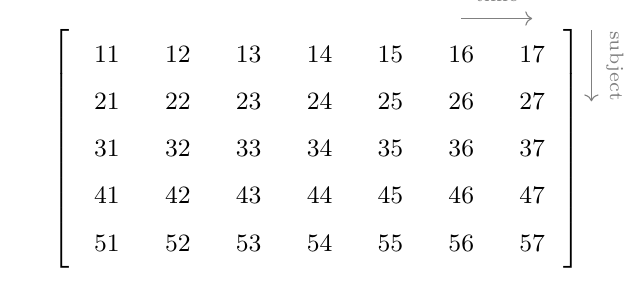
\begin{tikzpicture}
[   on grid,
    font = \small,
    baseline = -.7ex,
    inner sep=1pt,
    outer sep=0pt,
    minimum width=9mm,
    minimum height=6mm,
    every left delimiter/.style={xshift=2.5ex},
    every right delimiter/.style={xshift=-3.0ex}
]
\matrix (pred) [
	matrix of math nodes, 
    left delimiter={[}, 
    right delimiter={]},
]{ 
\y{1}{1} & \y{1}{2} & \y{1}{3} & \y{1}{4} & \y{1}{5} & \y{1}{6} & \y{1}{7} \\
\y{2}{1} & \y{2}{2} & \y{2}{3} & \y{2}{4} & \y{2}{5} & \y{2}{6} & \y{2}{7} \\
\y{3}{1} & \y{3}{2} & \y{3}{3} & \y{3}{4} & \y{3}{5} & \y{3}{6} & \y{3}{7} \\
\y{4}{1} & \y{4}{2} & \y{4}{3} & \y{4}{4} & \y{4}{5} & \y{4}{6} & \y{4}{7} \\
\y{5}{1} & \y{5}{2} & \y{5}{3} & \y{5}{4} & \y{5}{5} & \y{5}{6} & \y{5}{7} \\
};
\useasboundingbox[anchor=center] (pred.north west) rectangle (pred.south east);
\draw[->, black!50] ([xshift=2ex] pred-1-7.north east) -- ([xshift=2ex] pred-2-7.east)
    node [midway, font=\scriptsize, above, sloped] {subject};
\draw[->, black!50] ([yshift=1ex] pred-1-6.north) -- ([yshift=1ex] pred-1-7.north)
    node [midway, font=\scriptsize, above] {time};
\end{tikzpicture}
\end{equation}

Now, the indicator function can be computed 
using the defintion in \cref{eq:lh-indicator}
and the observed data \(\tid_i\) and \(\sigma_i\). 
In matrix form, the output of this function is
\begin{equation}
\bar{\bm{Y}}= \!\!\!\!
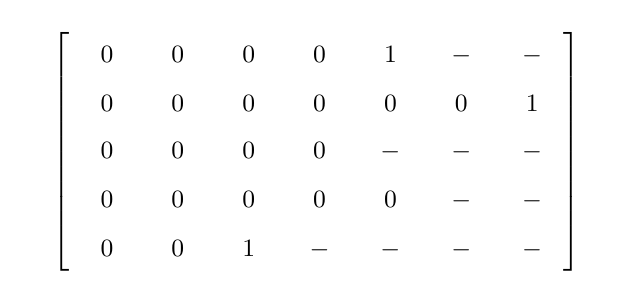
\begin{tikzpicture}
[   on grid,
    font = \small,
    baseline = -.7ex,
    inner sep=1pt,
    outer sep=0pt,
    minimum width=9mm,
    minimum height=6mm,
    every left delimiter/.style={xshift=2.5ex},
    every right delimiter/.style={xshift=-3.0ex}
]

\matrix (mask) [
	matrix of math nodes, 
    left delimiter={[}, 
    right delimiter={]}
]{ 
0 & 0 & 0 & 0 & 1 & - & - \\
0 & 0 & 0 & 0 & 0 & 0 & 1 \\
0 & 0 & 0 & 0 & - & - & - \\
0 & 0 & 0 & 0 & 0 & - & - \\
0 & 0 & 1 & - & - & - & - \\
};
\useasboundingbox[anchor=center] (mask.north west) rectangle (mask.south east);
\end{tikzpicture}
\end{equation}

Now, combining these two matrices according to the formula
in \cref{eq:lh-likelihood}, we obtain the likelihood in matrix form as
\begin{equation}
    \mathcal{L}(\bm{\hat{\Lambda}}, \bm{\bar{Y}}) = \!\!\!\!
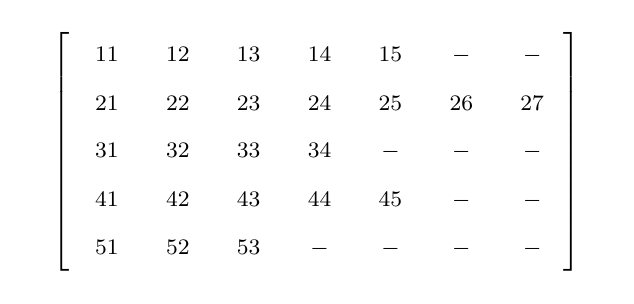
\begin{tikzpicture}
[   on grid,
    font = \small,
    baseline = -.7ex,
    inner sep=1pt,
    outer sep=0pt,
    minimum width=9mm,
    minimum height=6mm,
    every left delimiter/.style={xshift=2.5ex},
    every right delimiter/.style={xshift=-3.0ex}
]
\matrix (loss) [
	matrix of math nodes, 
    left delimiter={[}, 
    right delimiter={]},
    nodes={font=\footnotesize}
]{ 
\yy{1}{1} & \yy{1}{2} & \yy{1}{3} & \yy{1}{4} & \y{1}{5}  & -         & -         \\
\yy{2}{1} & \yy{2}{2} & \yy{2}{3} & \yy{2}{4} & \yy{2}{5} & \yy{2}{6} &  \y{2}{7} \\
\yy{3}{1} & \yy{3}{2} & \yy{3}{3} & \yy{3}{4} & -         & -         & -         \\
\yy{4}{1} & \yy{4}{2} & \yy{4}{3} & \yy{4}{4} & \yy{4}{5} & -         & -         \\
\yy{5}{1} & \yy{5}{2} & \y{5}{3}  & -         & -         & -         & -         \\
};
\useasboundingbox[anchor=center] (loss.north west) rectangle (loss.south east);
\end{tikzpicture}
\end{equation}
from which the log-likelihood, \cref{eq:lh-loglikelihood}, is then
\begin{equation*}
    \small
\begin{split}
    \mathscr{l}(\bm{\hat{\Lambda}}, \bm{\bar{Y}})
    &={} \log (\yy{1}{1}) + \log(\yy{1}{2}) + \log(\yy{1}{3}) + \log(\yy{1}{4}) 
     +  \log(\y{1}{5}) \\ 
    &+{} \log (\yy{2}{1}) + \log(\yy{2}{2}) + \log(\yy{2}{3}) + \log(\yy{2}{4}) 
     +  \log(\yy{2}{5}) + \log(\yy{2}{6}) +  \log(\y{2}{7}) \\
    &+{} \log (\yy{3}{1}) + \log(\yy{3}{2}) + \log(\yy{3}{3}) + \log(\yy{3}{4}) \\
    &+{} \log (\yy{4}{1}) + \log(\yy{4}{2}) + \log(\yy{4}{3}) + \log(\yy{4}{4}) 
    + \log(\yy{4}{5})  \\
    &+{} \log (\yy{5}{1}) + \log(\yy{5}{2}) + \log(\y{5}{3} )
\end{split}
\end{equation*}

\section{Survival Analysis with Competing Risks}

Up to this point, the description of concepts in survival analysis has
assumed the presence of only a single event type, such as all-cause mortality
(\cref{fig:ssm}).
In practice, particularly in clinical settings, 
this single-event model can be too restrictive,
and instead one needs to consider competing risks
(\cref{fig:msm}).
By definition, a competing risk is a secondary event whose occurence 
prevents the primary event from occuring.
For example,
in a study where the primary outcome is cardiovascular mortality,
deaths from non-cardiovascular causes are a competing risk.

\begin{marginfigure}[-10em]% →
    \tikzstyle{outcome}=[%
        rectangle, rounded corners, minimum height=5mm, fill=color3
    ]
    \centering
    \begin{tikzpicture}[x=0.60\linewidth, y=1cm]
    \graph [edge quotes={font=\scriptsize, fill=white}, 
            nodes      ={draw, outcome, sloped, minimum width=1cm}]{
        alive [fill=color4] -> dead [> "\(\lambda(t)\)" ];
    };
    \end{tikzpicture}
    \caption[Single-state survival model]{
        A simple survival analysis setup 
        involves modelling a single transition between states 
        \enquote{alive} and \enquote{dead}.
    }
    \label{fig:ssm}
\end{marginfigure}% ←

\begin{marginfigure}[0em]% →
    \tikzstyle{outcome}=[%
        rectangle, rounded corners, minimum height=5mm, fill=color3
    ]
    \centering
    \begin{tikzpicture}[x=0.60\linewidth, y=0.85cm]
    \graph [edge quotes={font=\scriptsize, fill=white}, 
            nodes      ={draw, outcome, sloped, minimum width=1cm}]{
        alive [fill=color4] -> {
            cause 1 [> "\(\lambda_1(t)\)" ],
            cause 2 [> "\(\lambda_2(t)\)" ],
            cause k [> "\(\lambda_\kappa(t)\)" ],
        };
    };
    \end{tikzpicture}
    \caption[Multi-state survival model]{
        A survival analysis setup with competing risks
        involves modelling transitions between states 
        \enquote{alive} and \(k\) different absorbing
        states, \enquote{cause 1} to \enquote{cause \(\kappa\)}
    }
    \label{fig:msm}
\end{marginfigure}% ←

\subsection{Cause-Specific Survival Quantities}

To describe time-to-event phenomena with competing risks, 
we introduce the cause-specific hazard function and 
cumulative-incidence function.
With \(R \in \{1, \dots, \kappa\}\) denoting the \(\kappa\) different competing risks, 
the continuous cause-specific hazard function is defined as
\begin{equation}
    \lambda_r(t) = \lim_{\Delta t \to 0} 
        \frac{\PR (t \leq T < t + \Delta t, R=r \mid T \geq t)}{\Delta t}
\end{equation}
where \(r\) refers to a specific value of \(R\).
The cause-specific cumulative incidence function is defined as
~\autocite{kalbfleischStatistical2002}
\begin{equation}
    F_r(t) = \PR(T \leq t, R = r).
\end{equation}

The overall hazard and cumulative incidence, 
which combines failures of any of the \(\kappa\) causes,
correspond to the hazard function 
and the cumulative distribution function 
in the single-event setting, that is
\begin{equation}
    \lambda(t) = \sum_{r=1}^{\kappa} \lambda_r(t)
    \quad \text{and} \quad
    F(t) = \sum_{r=1}^{\kappa} F_r(t).
\end{equation}

\subsection{Modelling the Cause-Specific Hazard}

In the competing risks setting, 
the typical approach is to treat competing risks as censored events
and use Cox regression to estimate the cause-specific hazards.
In this approach, the cause-specific hazard takes the form of
\begin{equation}
    \hat{\lambda}_{r}(t \giv \vec{x}) 
        = \lambda_{0r} \exp(\bm{\beta}_r \cdot \bm{x})
\end{equation}
from which one can obtain the cause-specific regression coefficients 
\(\bm{\beta}_r\).
In \studyi{}, we use this to estimate the cause-specific hazards
of \ac{IHD} progression and non-\ac{IHD} mortality associated with 
different clusters of \ac{IHD} patients, 
as defined by their respective comorbidity profiles.

However, an important assumption required by all survival methods
outlined so far, including the Cox proportional hazards model,
is that of noninformative censoring.
~\autocite{kleinbaumSurvival2011}
This assumption states that the
\textquote[kleinbaumSurvival2011]{%
    probability of being censored at time \(t\) does not depend on
    prognosis for failure at time \(t\)%
}, which in the context of competing risks can be especially problematic,
since it also implies that competing failure types should be independent.
It is difficult to ascertain if this is the case from observed data, 
however if we include risk-factors that are shared by competing events,
it is possible to alleviate the bias related to this possibly erroneous
assumption.
~\autocite{kleinbaumSurvival2011}

\subsection{The Aalen-Johansen Estimator}

In estimation of the population-level cause-specific incidence,
the approach of simply treating competing events as censored 
and applying the standard Kaplan-Meier estimator, 
is generally a bad idea, since it often leads to a very biased estimate of 
\(F(t)\).
~\autocite{pepeKaplan1993}
Instead, an alternative approach is the Aalen-Johansen estimator
that allows estimation of the cause-specific cumulative incidence.
~\autocite{aalenEmpirical1978}
Of note, the Aalen-Johansen is a general method for estimating
transition probabilities in state-transition models,
and can be used to describe complex multi-state models,
including those with repeated events and with non-terminal states.
~\autocite{survival-package}
However, we will be assuming a standard competing-risk setting
with \(\kappa\) different terminal states, 
as depicted in \cref{fig:msm}.
 
If we again order the distinct failure times, 
corresponding to any cause, 
such that
\(t_{(1)} < t_{(2)} < \ldots < t_{(j)}\),
and update the definition of \(\bar{D}(j)\) to keep track of cause-specific
events, such that we have
\begin{equation}
\begin{aligned}
    \bar{D}(j, r) &= \card \{i \in \{1, \dots, n\} \mid t_i = t_{(j)}, r_i = r\} \\
    \bar{A}(j)    &= \card \{i \in \{1, \dots, n\} \mid t_i > t_{(j)}\}.
\end{aligned}
\end{equation}
Now, the Aalen-Johansen estimator of the cumulative incidence function
can be defined as 

\begin{equation}
    \widehat{F}_r(t)
    =   \sum_{j \mid t_{(j)} \leq t}{
        \!\!
        \widehat{S}(t_{(j-1)})
        \frac{\bar{D}(j, r)}{\bar{A}(j)}
    }
\end{equation}
  % [X]
\chapter{Overview of Data Resources}

Data stands as the cornerstone of both precision medicine and machine learning.
Its availability is crucial; without it, research in these
fields would be almost impossible. 
The emergence of high-throughput analyses and \acp{EHR} has 
led to a Cambrian explosion of the volume of data being generated,
which has the potential of revolutionizing the 
entire landscape of biomedical research. 
However, the sensitive nature of this data means
that access is frequently a major challenge, 
often serving as a major bottleneck in
many research endeavors.

In the context of the studies conducted for this thesis, I have been in the
privileged position of working within a research group where permissions, 
data access, and the necessary infrastructure were already well-established.
In terms of infrastructure, a key aspect of our data handling involved the use 
of a secure high-performance computing environment. 
This not only ensured the efficient processing of large datasets and 
training of large neural networks, 
but also maintained the highest standards of data security and
confidentiality, which are paramount in dealing with sensitive health records.
These aspects have been instrumental in enabling and driving 
the research and analyses presented in this thesis.

Focusing on the data itself,
this chapter aims to provide a comprehensive overview of the various data
sources utilized in the studies comprising this thesis. It details the
databases and registries that were accessed and analyzed,
highlighting how each contributed to the research. 

\section{The Danish Civil Registration System}

\Ac{CPR} is the central administrative register in Denmark,
and stores personal information on the entire Danish population,
including birth date, sex, addresses, vital status, 
and, importantly, a unique personal identification number, 
known as \enquote{\ac{CPR}-nummer} or \enquote{personnummer}.
~\autocite{schmidtDanish2014}
The \ac{CPR} number is assigned at birth or upon obtaining Danish citizenship, 
and have been in use since 1968.
As of January 2, 2014, 
\num{9484792} \ac{CPR} numbers were assigned.
~\autocite{schmidtDanish2014}
Of these \num{5685912} were \enquote{active},
and \num{3798880} were \enquote{non-active},
the latter primarily attributed to death and emigration.
~\autocite{schmidtDanish2014}

In Denmark, the \ac{CPR} number is as essential as a bicycle, 
required for opening a bank account, 
borrowing a library book, 
getting treated for appendicitis, and everything in between.
This widespread use, 
combined with the country's long-standing tradition
of organising and keeping record of detailed data in 
administrative databases and registries,
have enabled the construction of a large network
of interlinkable epidemiological resources.
~\autocite{schmidtDanish2019}
In this light, the whole nation can be utilized as a research cohort
as outlined by \textcite{frankEpidemiology2000} in a letter
to \textit{Science}.

\section{The Danish National Patient Register}

Of the Danish registries, \ac{LPR} is arguably one of the most important.
\ac{LPR}, or \enquote{Landspatientregisteret}, 
is a comprehensive clinical register that has
been instrumental for clinical research and administration in Denmark,
and serves multiple critical functions.
~\autocite{schmidtDanish2015}
Primarily, it underpins the Danish Health and Medicines Authority's hospital
statistics and is a main foundation for health economic calculations.
Additionally, the \ac{LPR} is instrumental in monitoring the
prevalence of various diseases and treatments. 
Furthermore, the registry plays a key role in
facilitating quality assurance of Danish healthcare services and provides
hospital physicians access to patients' hospitalization histories, enhancing
patient care and treatment efficacy.
~\autocite{schmidtDanish2015}
The register is updated monthly based on reports from the hospitals,
and has been collecting data continuously since 1977.
~\autocite{schmidtDanish2015}

\subsection{Content and Structure}

The \ac{LPR} encompasses a wide array of data on each individual, 
such as personal information, admission and discharge details, diagnoses, 
examinations, treatments including surgeries, information on accidents, 
and additional details concerning births. 
~\autocite{schmidtDanish2015}
The information in the register is organised in a
structured format with different data types being stored 
in distinct tables that can be linked following a 
specified relational data model.
~\autocite{lpr2dok}

This data model, referred to as \acsfont{LPR2},  
have remained largely unchanged since the release of the registry in 1977.
However, in early 2019, it underwent a significant overhaul to a 
new and refined data model, \acsfont{LPR3}.
~\autocite{nielsenLPR32018}
The \acsfont{LPR3} model addresses certain limitations of its predecessor, 
notably enabling the creation of more fine-grained patient care timelines. 
While the specifics of these improvements are beyond the scope of this thesis, 
it is important to note that the \acsfont{LPR3} model is not entirely 
backwards compatible with the \acsfont{LPR2} data model. 
Nevertheless, depending on the specific use case, 
it remains possible to create data extracts that are compatible
to one another.

\subsection{Classification of Diseases}

The highly structured data within the \ac{LPR} 
is coded using the national \acs{SKS} classification scheme (\enquote{\acl{SKS}}), 
a collection of Danish, international, and Nordic classification standards
maintained by the Danish Health Data Authority.
~\autocite{schmidtDanish2015}
These standards includes
the \acfi{NOMESCO} system for surgical procedures,
the \acfi{ATC} system for medication,
and the \acfi{ICD} system for diagnoses. 
~\autocite{schmidtDanish2015}

Focusing on diagnosis codes, 
the \ac{LPR} is currently using the \ac{ICD-10},
and have been doing so since the start of 1994
where it replaced the \acsu{ICD-8}.
~\autocite{schmidtDanish2015}
This transition can complicate longitudinal studies of disease occurence, 
but prior efforts by the Brunak group have succesfully
created a mapping between \ac{ICD-8} and \ac{ICD-10}
that can be used to mitigate such challenges.
~\autocite{pedersenUnidirectional2023}

The \ac{ICD-10} coding system follows a hierarchical structure 
with every code beginning with a letter followed by two or more digits.
Each code falls in one of 21 high-level categorisation of diagnoses 
that e.g.  includes chapters
(ii)~\emph{Neoplasms};
(iv)~\emph{Endocrine, Nutritional, and Metabolic Diseases};
and (ix)~\emph{Diseases of the Circulatory System}.
Using the latter as an example, 
\cref{fig:icd10-hierarchy} shows the hierarchical structure of the
\ac{ICD-10}.

% figure: icd10-hierarchy→
\begin{figure}
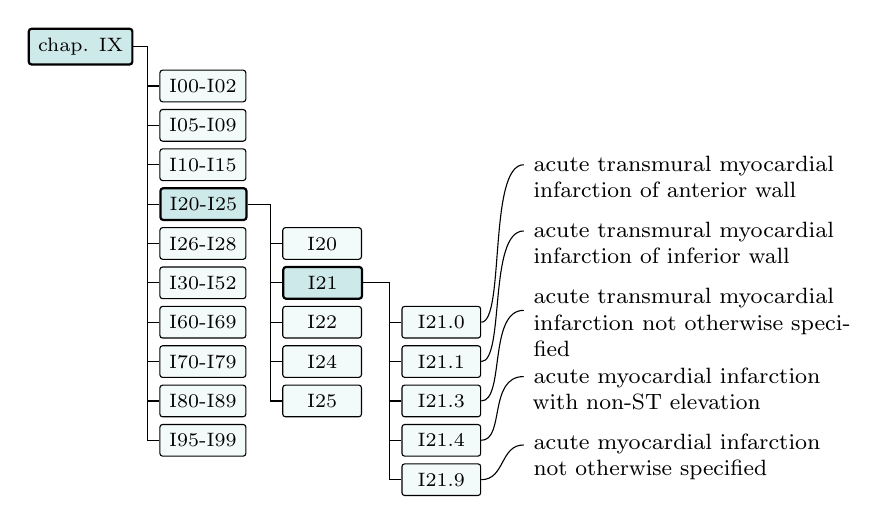
\begin{tikzpicture}[
    every node/.append style = {
        draw, anchor = west, 
        minimum width=10mm, 
        minimum height=4mm,
        font=\tlfstyle\scriptsize,
        rounded corners=1pt,
        fill=color2!5
    },
    sel/.style = {fill=color2!20, draw=black, thick},
    txt/.style = {
        fill=none, draw=none, font=\footnotesize, text width=4.0cm,
        text height=5mm
    },
    grow via three points={
        one child    at (1.0, -0.5) and 
        two children at (1.0, -0.5) 
                    and (1.0, -1.0)
    },
    edge from parent path={
        (\tikzparentnode.east) 
        -| ([xshift=-4.2]\tikzchildnode.west)
        |- (\tikzchildnode.west)
    }]
    \node[sel] {chap. IX}
        child {node {I00-I02}}
        child {node {I05-I09}}
        child {node {I10-I15}}
        child {node[sel] {I20-I25}
            child {node (i20) {I20}}
            child {node [sel] (i21) {I21}
                child {node (1) {I21.0}}
                child {node (2) {I21.1}}
                child {node (3) {I21.3}}
                child {node (4) {I21.4}}
                child {node (5) {I21.9}}
            }
            child {node {I22}}
            child {node {I24}}
            child {node {I25}}
        }
        child {node {I26-I28}}
        child {node {I30-I52}}
        child {node {I60-I69}}
        child {node {I70-I79}}
        child {node {I80-I89}}
        child {node {I95-I99}}
    ;

    \node [txt] (t1) at (6.3cm, -1.5cm) 
        {acute transmural myocardial infarction of anterior wall};
    \node [txt, below=3mm of t1.center] (t2) 
        {acute transmural myocardial infarction of inferior wall};
    \node [txt, below=3mm of t2.center] (t3) 
        {acute transmural myocardial infarction not otherwise specified};
    \node [txt, below=3mm of t3.center] (t4) 
        {acute myocardial infarction with non-ST elevation};
    \node [txt, below=3mm of t4.center] (t5) 
        {acute myocardial infarction not otherwise specified};

    \draw (1.east) .. controls +(2ex,0) and +(-3ex,0) .. (t1.west);
    \draw (2.east) .. controls +(2ex,0) and +(-3ex,0) .. (t2.west);
    \draw (3.east) .. controls +(2ex,0) and +(-3ex,0) .. (t3.west);
    \draw (4.east) .. controls +(2ex,0) and +(-3ex,0) .. (t4.west);
    \draw (5.east) .. controls +(2ex,0) and +(-2ex,0) .. (t5.west);
    
\end{tikzpicture}
\caption[The ICD-10 Hierarchy]{%
    Schematic illustrating the hierarchical structure of the \ac{ICD-10} coding
    system. 
    Using Chapter IX---which covers diseases of the circulatory system
    (codes I00-I99) and comprises ten different \enquote{blocks}---as an example, 
    the diagram shows how these blocks are segmented into 
    \enquote{level 3} codes, such as I20 to I25, 
    corresponding to ischemic heart disease. 
    It provides an expanded view of the I21 category, 
    containing specific subtypes, \enquote{level 4} codes, 
    of acute myocardial infarctions 
    from I21.0 for the anterior wall 
    to I21.9 for unspecified instances. 
    Deeper levels of the hierarchy also exists,
    but is not included in this diagram.
}
\label{fig:icd10-hierarchy}
\end{figure}
% ←

\section{The East Danish Heart Registry}

\ac{RKKP} is a program set in place to support the
management and infrastructure related to clinical quality databases.


Data from some of the other general registries, 
including the \ac{LPR}, is being used to populate 
specific variables in different \ac{RKKP} registries.

The \ac{RKKP} undergoes revision by the National Health Authority
every three years to continuously assess specific 
criteria for function, safety, and methodology.


\section{The Register of Pharmaceutical Sales}



\section{The Causes of Death Register}

When a person in Denmark dies, a doctor performs a post-mortem examination. The
doctor fills in a death certificate and reports the death by submitting the
certificate to the Danish Health Authority.

\section{The BigTempHealth Project}

\subsection{Patient Notes}

The DNPR does not contain information on tobacco usage, blood pressure, 
body-mass index, and other important covariates to consider in the
context of cardiovascular diseases.

% figure: journal text→
\begin{figure}
{
% Define new commands for each category
\newcommand{\cbox}[2]{%
    \tcbox[on line, colback=#1!50!white, boxsep=1.5pt, colframe=black,
           valign=center, left=0pt, right=0pt, top=0pt, bottom=0pt, boxrule=1pt]{#2}%
}%
\newcommand{\diag}[1]{\cbox{color3}{#1}}
\newcommand{\symp}[1]{\cbox{color4}{#1}}
\newcommand{\drug}[1]{\cbox{color5}{#1}}
\newcommand{\quan}[1]{\cbox{color6}{#1}}
\newcommand{\kwpa}[1]{\cbox{color7}{#1}}

\begin{Verbatim}[commandchars=\\\{\}, fontsize=\scriptsize, 
    frame=single, framesep=1em, numbers=left, numbersep=3pt]
68-year-old woman, no earlier known cardiovascular disease, 
referred by gp for observation of \diag{angina pectoris}.

Risk factors:
\diag{Hypertension}: Yes, newly discovered, currently well-treated.
\diag{Hypercholesterolemia}: Yes. Under treatment.
Family: No family history of \diag{ischemic heart disease}.
Smoking: Quit 15 years ago, before that 20 pack-years.
Claudication: No.

Previously:
Known since 2001 with \diag{type II diabetes mellitus}, treated 
with \drug{Metformin}.  Followed up with regular checks. 
Complications with discrete neuropathy and beginning 
macular degeneration.

Currently:
For about 3 months, \symp{intermittent pressure in the left side}
\symp{of the chest}. No radiation, independent of physical 
activity. Daily attacks lasting a few seconds. During the 
same period, has been diagnosed with \diag{severely elevated blood}
\diag{pressure}. Recently started anti-hypertensive treatment with
good effect.

Medication:
- \drug{Metformin} \quan{1000 mg} x 2
- \drug{Simvastatin} \quan{20 mg} x 1
...

Objective:
Normal general condition.
Nutritional status above average.
\kwpa{Blood pressure 149/91}, \kwpa{pulse 76}, \kwpa{height 177 cm}, \kwpa{weight 96 kg}
\end{Verbatim}
}
\caption{Artificial example of unstructured text in an \ac{EHR}}
\end{figure}% ←
    % [ ]


\part{Outline of Studies}
% \chapter{Paper 1: Multimorbidity Clustering in Ischemic Heart Disease}
\label{chap:outline-paper-1}

Describe clustering methods.

\section{Related Work}

     % [ ]
% \chapter{Study II: Time-to-Event Prediction of All-Cause Mortality}
\label{outline-study-2}
     % [ ]
% \chapter{Study III: Time-to-Event Prediction with Competing Risks}
\label{outline-study-3}

\section{Model formulation}

The proposed model parametrizes the cause-specific conditional hazards,
and the output \(\Lambda\) is then a 
\(n \times q \times (m + 1)\) matrix of probabilities
where values across the last dimension all sum up to 1.


In the case of several competing target events,
it is necessary to define several hazard functions,
one for each distinct outcome type.
Let \(R \in \{1, ..., m\}\) denote the competing risks.
Then, for disrete time \(T \in \{1, ..., q\}\), 
the cause-specific hazard function from cause $r$ is defined by
%
\begin{equation*}
    \lambda_{r}(t | \mathbf{x}) = \Pr (T = t, R = r | T \geq t, \mathbf{x})
\end{equation*}
%
where \(\mathbf{x}\) is a vector of time-independent predictor variables. 
The different hazard functions, 
\(\lambda_{1}(t|\mathbf{x}), ..., \lambda_{m}(t|\mathbf{x})\) 
can be combined into the overall hazard function defined as
%
\begin{equation}
    \lambda(t|\mathbf{x}) 
    = \sum_{r=1}^{m}(\lambda_{r}(t|\mathbf{x}))
    = \Pr(T = t | t \leq T, \mathbf{x})
\end{equation}
%
From this it follows that the survival function is
%
\begin{equation}
    S(t|\mathbf{x})
    = \Pr(T >= t|\mathbf{x})
    = \prod_{i=1}^{t}(1 - \lambda(i|\mathbf{x}))
\end{equation}

The model uses $m + 1$ categorical responses.
The responses are either any of the $m$ competings risks, 
or conditional survival.
%
\begin{equation}
    \Pr(T > t | T \geq t, \mathbf{x})
    = 1 - \sum_{r = 1}^{m} \lambda_r (t | \mathbf{x})
    = 1 - \lambda (t | \mathbf{x})
\end{equation}

\section{Model formulation}

Continuous follow-up time is divided into into $q$ intervals
%
\begin{equation*}
	[0, a_1), [a_1, a_2), ..., [a_{q-1}, a_q), [a_{q}, \infty)
\end{equation*}
%
and the time to event variable \(T\) is denoted 
with a positive integer \(t = 1, 2, ...\),
which points to the interval \([a_{t-1}, a_{t})\).
With this discrete time scale,
the cause specific hazard function \(\lambda_{r}(t)\) is a conditional probability defined as
%
\begin{equation*}
    \lambda_{r}(t | \mathbf{x}) = \Pr (T = t, R = r | T \geq t, \mathbf{x})
\end{equation*}
%
given a vector \(\mathbf{x}\) of predictor variables.

The discrete hazard function is defined as
the probability of failure in the interval \(t\),
given that the individual is still alive at the end of the preceding interval
\(t - 1\).

In a time-to-event model with several competing target events,
we describe the process with multiple hazard functions, 
that each describe a specific target outcome or risk.
Typically, 
we refer to the individual hazard functions as cause-specific hazards.

For discrete time \(T \in \{1, ..., s+1\}\), and with a given vector \(\mathbf{x}\) of time-independent covariates,
the cause-specific hazard from cause \(r\) is defined as

\begin{equation}
    \lambda_{r}(t|\mathbf{x}) 
    = P(T = t, R = r | t \leq T, \mathbf{x})
\end{equation}

Which represents the probability of 

The overall hazard function is

\begin{equation}
    \lambda(t|\mathbf{x}) 
    = \sum_{r=1}^{m}(\lambda_{r}(t|\mathbf{x}))
    = P(T = t | t \leq T, \mathbf{x})
\end{equation}

The survival function is the unconditional probability of an event in period \(t\) given the specific covariates is 

\begin{equation}
    S(t|\mathbf{x})
    = P(T >= t|\mathbf{x})
    = \prod_{i=1}^{t}(1 - \lambda(i|\mathbf{x}))
\end{equation}

From the hazard we can obtain the survival function 
%
\begin{equation*}
    S(t | \mathbf{x}) 
    = \Pr (T \geq t | \mathbf{x}) 
    = \prod_{s = 1}^{t-1} (1 - \lambda(s | \mathbf{x}))
\end{equation*}
%
which represents the unconditional probability of surviving interval \(t\) given the specific covariates cf. \autocite{tutzModeling2016}.

Of note, this interpretation is considerably more accessible than the usual
continuous hazard one.


\begin{equation}
    S(\tau) = P(T > \tau) = \sum_{i = 1}^{\tau - 1} (P(T = \tau - i))    
\end{equation}

The cause specific cumulative incidence function is

\begin{equation}
	CIF_r(t|\mathbf{x})
	= \sum_{i=1}^{t}\lambda_{r}(t|\mathbf{x}) S(t-1|\mathbf{x})
\end{equation}

Let the data be given by \(t_{i}, r_{i}, \delta_{i}, \mathbf{x}_{i}\),
where \(r_{i} \in \{1, ..., m\}\) indicates the target event. 
Assuming random censoring at the end of the interval
with \(t_i = \min\{T_i, C_i\}\), 
where events are defined by the indicator function

\begin{equation}
\delta_i = 
	\begin{cases}
		1, & T_i \leq C_i \\
		0, & T_i > C_i
	\end{cases}
\end{equation}

\begin{subequations}
\begin{equation}
	nll =
	- \sum_{i=1}^{n}
	\sum_{t=1}^{ti}
	\left(
		\sum_{r \in C} \delta_{itr} \log(\lambda_{r} (t | \mathbf{x}))
		+ \delta_{it0} \log\left(
			1 - \sum_{r \in C} \lambda_{r} (t | \mathbf{x})
		\right)
	\right)
\end{equation}

Or alternatively 

\begin{equation}
	nll =
	- \sum_{t=1}^{q}
	\sum_{i \in R_s}
	\delta_{is} \log(s|\mathbf{x}_i) 
	+ (1 - \delta_{is}) (1 - \log(s|\mathbf{x}_i)))
\end{equation}
\end{subequations}

In our approach, the neural network parametrises the logistic hazards.
The goal is to learn \( \hat{h}(t | \mathbf{x}) \)
for each of the competing events.




The discrete probability function

\begin{equation}
    f_l = \Pr (T \in A_l) = S(t_{l-1}) - S(t|l)
\end{equation}

the discrete hazard rate

\begin{equation}
    h_l = \Pr (T \in A_l | T > t_{l-1}) = \frac{f_l}{S(t_{l-1})}
\end{equation}

    
The contribution to the likelihood function of the \textit{i}th subject

For uncensored subjects, the contribution is
%
\begin{equation}
    \Pr (T_i \in A_{l_i}) = f_{l_i} = h_{l_i} \prod_{l=1}^{l_i-1}(1-h_{l_i})
\end{equation}
%
while for censored subject, the contribution is
%
\begin{equation}
    \Pr (T_i > t_{l_i}) = S(t_{l_i}) = \prod_{l=1}^{l}(1-h_{l_i})
\end{equation}

A similar approach have previously been described \autocite{biganzoliFeed1998}.

     % [ ]

\part{Discussion}
\chapter{Conclusions and Future Perspectives}
\label{conclusions}



Leveraging population-level genomic datasets from large biobanks,
it should be possible to implement genetics informed risk stratification
for routine clinical use.


\section{Topics to be discussed}
\begin{itemize}
    \item Consider doing ablation studies to produce less-complex versions
        of the predictions models.
    \item Lack of prospective validation of medical prediction models
    \item Lack of clinical deployment and adoption 
    \item Limitations of explainable AI
\end{itemize}


        % [ ]
% 
\chapter*{Misc}

A specific chromosomal translocation in 
chronic myeloid leukemia (CML) 
results in a constitutively active tyrosine-kinase (BCR-ABL)
that can be targeted with tyrosine kinase inhibitors such as imatinib~%
\autocite{drukerEfficacy2001}.

%------------------------------------------------------------------------
\vskip 5em

For predictive models to be effective,
they must enable clinicians to guide treatment by:
%
\begin{enumerate*}
    \item providing actionable insights on modifiable risk factors
    \item being adapted to the individual patient
    \item being generally applicable in different populations
\end{enumerate*}

%------------------------------------------------------------------------
\vskip 5em

AI-driven medical prediction models are able to synthesize large amounts
of electronic health data into risk scores or estimates that can be used
to assess the risk and condition of the individual patient~\autocite{handelmanEDoctor2018}.

%------------------------------------------------------------------------
\vskip 5em

\begin{itemize}
    \item Draw illustration of overfitting. Some sort of classifier with a
        super irregular decision boundary.
\end{itemize}

%------------------------------------------------------------------------
\vskip 5em


Complications also occur in otherwise asymptomatic patients, 
and for that reason risk evaluation should apply to both patients
with out without symptoms.
~\autocite{knuuti20192020}

Although revascularization can relieve symptoms for the culprit lesions
responsible for myocardial ischemia, it may not prevent the progression
of other neighboring lesions and future acute thrombotic events.
~\autocite{libbyPathophysiology2005}

\textquote[byrne20232023]{%
    A number of prognostic models \textelp{}
    have been formulated into clinical risk scores and, among
    these, the GRACE risk score offers the best discriminative performance and
    is therefore recommended for risk assessment.%
}

\textquote[knuuti20192020]{% class I recommendation
    Invasive coronary angiography is recommended as an alternative test to
    diagnose \textsc{CAD} \textins{coronary artery disease} in patients with a high
    clinical likelihood, severe symptoms refractory to medical therapy or
    typical angina at a low level of exercise, and clinical evaluation that
    indicates high event risk.%
}

\textquote[knuuti20192020]{% class IIa recommendation
    Invasive coronary angiography with the availability of invasive functional
    evaluation should be considered for confirmation of the diagnosis of CAD in
    patients with an uncertain diagnosis on non-invasive testing%
}

Myocardial tissue damage can be detected with high sensitivity by measuring 
the release troponins and creatinine-kinase from the sarcolemma.
~\autocite{falkPathogenesis2006}

The esc guidelines on risk-prevention highlights 
that one of the currents gaps in evidence,
is comparing the performance of competing risk-adjusted 
cardiovascular disease risk models versus the standard models.
~\autocite{visseren20212021}


\bookmarksetup{startatroot}

\backmatter %%%%%%%%%%%%%%%%%%%%%%%%%%%%%%%%%%%%%%%%%%%%%%%%%%%%%%%%%%%%%%%%%%%

\addcontentsline{toc}{chapter}{List of References}
\printbibliography

\mainmatter %%%%%%%%%%%%%%%%%%%%%%%%%%%%%%%%%%%%%%%%%%%%%%%%%%%%%%%%%%%%%%%%%%%

\appendix
\appendixpage
\addappheadtotoc
\cleardoublepage

\includepdf[
    clip, trim=1cm 6cm 1cm 1.8cm, offset=0 -2.2cm, 
    frame=true, scale=0.8, pages=1, 
    pagecommand=\chapter{Manuscript for Study I}\label{chap:paper-1}]%
    {assets/paper1-clustering.pdf}

% \includepdf[
%     clip, trim=1cm 0 1cm 1.5cm, offset=0 0, 
%     frame=true, scale=0.8, 
%     pages=2-, pagecommand={}]%
%     {assets/paper1-clustering.pdf}

\cleardoublepage
\includepdf[
    clip, trim=1cm 6cm 1cm 1.8cm, offset=0 -2.2cm, 
    frame=true, scale=0.8, pages=1, 
    pagecommand=\chapter{Manuscript for Study II}\label{chap:paper-2}]%
    {assets/paper1-clustering.pdf}

\cleardoublepage
\includepdf[
    clip, trim=1cm 6cm 1cm 1.8cm, offset=0 -2.2cm, 
    frame=true, scale=0.8, pages=1, 
    pagecommand=\chapter{Manuscript for Study III}\label{chap:paper-3}]%
    {assets/paper1-clustering.pdf}

\end{document}
